\documentclass[11pt]{formatting-template}

% mathptmx is a Times Roman look-alike (don't use the times package)
% It isn't clear if Times is required. The OGS manual lists several
% "standard fonts" but never says they need to be used.
% \usepackage{mathptmx}

\usepackage[NoDate]{currvita}
\usepackage{array}
\usepackage{tabularx}
\usepackage{booktabs}
\usepackage{ragged2e}
\usepackage{microtype}
\usepackage[breaklinks=true,pdfborder={0 0 0}]{hyperref}
\usepackage{graphicx}
\AtBeginDocument{%
	\settowidth\cvlabelwidth{\cvlabelfont 0000--0000}
}

% OGS recommends increasing the margins slightly.
\increasemargins{.1in}

\usepackage[english]{babel}
\usepackage{blindtext}

\usepackage{url}

\usepackage[super,sort&compress]{natbib}

\overfullrule5pt

%%%%%%%%%%%%%%%%%%%%%%%%%%%%%%%%%%%%%%%%%%%%%%%%%%%%%%%%%%%%%%%%%%%%%%%%%%%%%%%%
% Thesis Title & Author Information
\title{My title here}
\author{Author Name}
\degree{Bioinformatics \& Systems Biology}{Doctor of Philosophy}

% Thesis Committee Members
\chair{Professor One}
\cochair{Professor Two} 
\committee{Professor Three}
\committee{Professor Four} % alphabetical order required
\committee{Professor Five}
\degreeyear{2023}

%%%%%%%%%%%%%%%%%%%%%%%%%%%%%%%%%%%%%%%%%%%%%%%%%%%%%%%%%%%%%%%%%%%%%%%%%%%%%%%%
\begin{document}

% Begin with front matter and so forth
\frontmatter
\maketitle{}
\makecopyright{}
\makesignature{}

%%%%%%%%%%%%%%%%%%%%%%%%%%%%%%%%%%%%%%%%%%%%%%%%%%%%%%%%%%%%%%%%%%%%%%%%%%%%%%%%
% Dedication
%%%%%%%%%%%%%%%%%%%%%%%%%%%%%%%%%%%%%%%%%%%%%%%%%%%%%%%%%%%%%%%%%%%%%%%%%%%%%%%%
\begin{dedication}
	\setsinglespacing{}
	\parindent0pt\parskip\baselineskip{}
	\vskip0pt plus.25fil
	\begin{center}
		
		$\cdots$

		This dissertation is dedicated to \dots\\
		and \textit{Person}.
		
	\end{center}
\end{dedication}

%%%%%%%%%%%%%%%%%%%%%%%%%%%%%%%%%%%%%%%%%%%%%%%%%%%%%%%%%%%%%%%%%%%%%%%%%%%%%%%%
% Epigraph
%%%%%%%%%%%%%%%%%%%%%%%%%%%%%%%%%%%%%%%%%%%%%%%%%%%%%%%%%%%%%%%%%%%%%%%%%%%%%%%%
\begin{epigraph}
	\vskip0pt plus.5fil
	\vfil\vfil
	\setsinglespacing{}
	{ \flushright{
		This is an epigraph\\
		about epigraphs.\\
		}
		\vskip\baselineskip{}
		- \textit{Author Name}\par
	}
	\vfil\vfil\vfil
\end{epigraph}

%%%%%%%%%%%%%%%%%%%%%%%%%%%%%%%%%%%%%%%%%%%%%%%%%%%%%%%%%%%%%%%%%%%%%%%%%%%%%%%%
% Table of Contents, Figures, Tables, Etc.
%%%%%%%%%%%%%%%%%%%%%%%%%%%%%%%%%%%%%%%%%%%%%%%%%%%%%%%%%%%%%%%%%%%%%%%%%%%%%%%%
% Next comes the table of contents, list of figures, list of tables,
% etc. If you have code listings, you can use \listoflistings (or
% \lstlistoflistings) to have it be produced here as well. Same with
% \listofalgorithms.

\tableofcontents
\listoffigures
\listoftables

%%%%%%%%%%%%%%%%%%%%%%%%%%%%%%%%%%%%%%%%%%%%%%%%%%%%%%%%%%%%%%%%%%%%%%%%%%%%%%%%
% Acknowledgements
%%%%%%%%%%%%%%%%%%%%%%%%%%%%%%%%%%%%%%%%%%%%%%%%%%%%%%%%%%%%%%%%%%%%%%%%%%%%%%%%
\begin{acknowledgements}
	I would like to thank the following people for their support throughout my graduate school journey. \textit{Professor One} for being a great advisor. \textit{Professor Two} for being a great co-advisor. \textit{Professor Three} for being a great committee member. \textit{Professor Four} for being a great committee member. \textit{Professor Five} for being a great committee member. \textit{Professor Six} for being a great committee member. \textit{Professor Seven} for being a great committee member. \textit{Professor Eight} for being a great committee member. \textit{Professor Nine} for being a great committee member. \textit{Professor Ten} for being a great committee member. \textit{Professor Eleven} for being a great committee member. \textit{Professor Twelve} for being a great committee member. \textit{Professor Thirteen} for being a great committee member. \textit{Professor Fourteen} for being a great committee member. \textit{Professor Fifteen} for being a great committee member. \textit{Professor Sixteen} for being a great committee member. \textit{Professor Seventeen} for being a great committee member. \textit{Professor Eighteen} for being a great committee member. \textit{Professor Nineteen} for being a great committee member. \textit{Professor Twenty} for being a great committee member. \textit{Professor Twenty-One} for being a great committee member. \textit{Professor Twenty-Two} for being a great committee member. \textit{Professor Twenty-Three} for being a great committee member. \textit{Professor Twenty-Four} for being a great committee member. \textit{Professor Twenty-Five} for being a great committee member. \textit{Professor Twenty-Six} for being a great committee member. \textit{Professor Twenty-Seven} for being a great committee member. \textit{Professor Twenty-Eight} for being a great committee member. \textit{Professor Twenty-Nine} for being a great committee member. \textit{Professor Thirty} for being a great committee member. \textit{Professor Thirty-One} for being a great committee member. \textit{Professor Thirty-Two} for being a great committee member. \textit{Professor Thirty-Three} for being a great committee member.
\end{acknowledgements}

%%%%%%%%%%%%%%%%%%%%%%%%%%%%%%%%%%%%%%%%%%%%%%%%%%%%%%%%%%%%%%%%%%%%%%%%%%%%%%%%
% Vita
%%%%%%%%%%%%%%%%%%%%%%%%%%%%%%%%%%%%%%%%%%%%%%%%%%%%%%%%%%%%%%%%%%%%%%%%%%%%%%%%
\begin{vita}
\noindent
\begin{cv}{}
\begin{cvlist}{}
	\item[2012] High School Diploma\\
		University City High School
	\item[2012--2016] B.S. in Usefulology\\
		University of California, San Diego
	\item[2016--2023] Ph.D. in Bioinformatics \& Systems Biology\\
		University of California, San Diego
\end{cvlist}
\end{cv}

%%%%% PUBLICATIONS %%%%%
\publications{}

\noindent \textit{Author names marked with $\dagger$ indicate shared first co-authorship.} \newline
\noindent \textit{Publications marked with $\triangle$ are included in this text.} \newline

\noindent \textbf{Author Name} and Professor One. ``My first publication.'' \textit{Journal of Publications}, 2020. $\triangle$ \newline

%%%%% FIELDS OF STUDY %%%%% 
% This section was omitted within this thesis as it was optional.

\end{vita}

%%%%%%%%%%%%%%%%%%%%%%%%%%%%%%%%%%%%%%%%%%%%%%%%%%%%%%%%%%%%%%%%%%%%%%%%%%%%%%%%
% Dissertation Abstract 
%%%%%%%%%%%%%%%%%%%%%%%%%%%%%%%%%%%%%%%%%%%%%%%%%%%%%%%%%%%%%%%%%%%%%%%%%%%%%%%%
\begin{dissertationabstract}
	An abstract should provide a clear impression of the content and major divisions of the dissertation or thesis. Abstracts of doctoral dissertations must not exceed 350 words. 
\end{dissertationabstract}

%%%%%%%%%%%%%%%%%%%%%%%%%%%%%%%%%%%%%%%%%%%%%%%%%%%%%%%%%%%%%%%%%%%%%%%%%%%%%%%%
% Main Text of the Dissertation
%%%%%%%%%%%%%%%%%%%%%%%%%%%%%%%%%%%%%%%%%%%%%%%%%%%%%%%%%%%%%%%%%%%%%%%%%%%%%%%%
\mainmatter{}

\begin{dissertationintroduction}
    
\setcounter{chapter}{0}
\chapter*{Introduction}

\label{chap:introduction}

\section{The importance of RNA localization}
The fundamental unit of life is the cell, from unicellular organisms like bacteria to complex multicellular organisms like humans. While it is convenient to think of cells as amorphous liquid bags of lipids, proteins and sugars, cells are highly structured and and regulated. The genome serves as the template for RNAs; they are synthesized then modified by tightly orchestrated processes such as splicing, localization, translation, and degradation so a cell can function. We can measure the abundance of a cell's transcriptome, the complete repertoire of RNA, to loosely quantify cellular activity. But what do these molecules physically interact with? Where do these interactions occur in the cell and what causes them to interact? This layer of regulation, RNA localization, plays an important role in cell processes such as protein synthesis, signaling pathways and RNA degradation. For example, mRNAs exhibit asymmetric distributions in developing \textit{Drosophila melanogaster} embryos, compartment-specific localization in the neurites of neurons, and colocalization with the actin cytoskeleton in fibroblasts \cite{buxbaumRightPlaceRight2015}. The prevalence of RNA localization across diverse cell types and organisms indicate that it is a highly conserved process. Abnormal RNA localization has also been associated with many neurodegenerative diseases such as Huntington's disease (HD), where defects in axonal mRNA transport and subsequent translation in human spiny neurons lead to cell death and neurodegeneration \cite{fernandopulleRNATransportLocal2021}. Despite these repeated observations, the determinants of localization are not well understood.

\section{Spatial transcriptomics technology}

While we can easily quantify RNA expression with sequencing, RNA imaging techniques have traditionally been limited to visualizing a handful of species per experiment. However, recent multiplexed imaging technologies have unlocked much higher experimental throughput at hundreds to thousands of species, enabling nearly transcriptome-scale analysis of spatial RNA distributions. Single-molecule fluorescent in situ hybridization\cite{rajImagingIndividualMRNA2008} (smFISH) was one of the first popularized techniques able to image RNAs by species using synthesized complementary DNA (cDNA) sequences with fluorochromes. The cDNA probes hybridize to RNA targets and emit light upon excitation, which is captured by microscope cameras as dots of light, less than a micron wide. By designing specific probes for each RNA species of interest, it is possible to image multiple unique species at a time in the same cells. In order to scale to target hundreds to tens of thousands of unique RNA species, recent combinatorial FISH techniques compress the number of imaging rounds needed to identify each target by designing sets of barcodes that fluoresce in a specific sequence of images for individual RNA species. For example, MERFISH\cite{chenSpatiallyResolvedHighly2015} is one technique using a barcoding scheme that allows detection of 10,000 unique RNA targets in 69 rounds of sequential images. At such a scale, we can begin to study the RNA life cycle from a new perspective, by observing the spatial organization of the transcriptome and uncovering principles of RNA regulation linked to localization. The set of technologies able to capture the spatial organization of RNA in cells and tissue is termed spatial transcriptomics.\footnote{In addition to imaging-based methods, there exists a host of slide-based methods that are just as prevalent but not in the scope of this work. In summary these methods use a grid of barcoded wells on slides to capture and sequence transcripts. The location of each well is used to spatially map transcripts.}

\section{Current analysis trends}

As spatial transcriptomics assays reaches the scientific main stream \cite{marxMethodYearSpatially2021}, there is a growing need for scalable analysis software and computational infrastructure. The most robust and enduring tools adhere to FAIR principles\cite{wilkinsonFAIRGuidingPrinciples2016} — Findability, Accessibility, Interoperability, and Reusability—a set of standards proposed by researchers to maximize reuse of research objects for advancing scientific discovery. Data management strategies such as version control, software containerization, and pipeline management are often second priority in academic research. Consequentially, many academic tools do not see use outside of their initial projects and collaborations due to low adoption. Mainstream media attention around the “reproducibility crisis” and high profile cases of academic fraud have demonstrated the clear value of enforcing FAIR principles for academic research, both to researchers and for building trust with the average citizen. 

The field of spatial transcriptomics has witnessed an evolution of various tools and platforms, each specializing in different aspects of analysis and data handling. For image processing, tools like \textit{multi-fish}\cite{wangEASIFISHThickTissue2021}, \textit{mcmicro}\cite{schapiroMCMICROScalableModular2022}, and \textit{MERlin}\cite{ZhuangLabMERlinMERlin} are tailored specifically for certain technologies. In contrast, \textit{starfish/PIPEFISH}\cite{othersStarfishOpenSource,cisarUnifiedPipelineFISH2023} and \textit{spotfish} (described in this work) attempt to be platform agnostic and focus on pipeline building infrastructure instead of task-specific algorithms. In terms of data structures, \textit{AnnData}\cite{virshupAnndataAnnotatedData2021} specifically supports single-cell data matrices, while \textit{SpatialData}\cite{marconatoSpatialDataOpenUniversal2023}, \textit{SpatialExperiment}\cite{righelliSpatialExperimentInfrastructureSpatiallyresolved2022} offer more complex representations, attempting supporting a spectrum of data modalities and the relationships between them. Single-cell analysis is the \textit{de facto} approach to analyze spatial transcriptomics, and tools such as \textit{Giotto}\cite{driesGiottoToolboxIntegrative2021}, \textit{Squidpy}\cite{pallaSquidpyScalableFramework2021}, \textit{Stereopy}\cite{STOmicsStereopy2023}, \textit{stLearn}\cite{phamStLearnIntegratingSpatial2020}, and \textit{Voyager}\cite{mosesVoyagerExploratorySinglecell2023} are equipped to handle cell-centric functional analyses. Subcellular analysis, which delves deeper into spatial interactions at the molecular level, features tools like \textit{INSTANT}\cite{kumarIntracellularSpatialTranscriptomic2023}, \textit{SpaGNN}\cite{fangSubcellularSpatiallyResolved}, and \textit{FISHfactor}\cite{walterFISHFactorProbabilisticFactor}. \textit{Bigfish}\cite{imbertFISHquantV2Scalable2022} and \textit{Bento}\cite{mahBentoToolkitSubcellular2022} in this category are examples of software packages developed with FAIR principles in mind. Overall, this brief listing highlights the growing interest in the budding field of spatial transcriptomics and the need for FAIR tools to support the maturation of the field.


\setlength\LTleft{0pt}
\setlength\LTright{0pt}
\begin{small}
    \renewcommand\thetable{0.1}
    \begin{landscape} % this table is long
        \begin{longtable}{l l l l l l l}
            % Define the table title in the table of contents
            \caption{Assessment of FAIR principles in spatial transcriptomics tools}\label{tab:spatial-tx tools assessment}
            \\ \hline 

            % Define the table columns for the first and all subsequent pages
            \multicolumn{1}{l}{\textbf{Category}} & \multicolumn{1}{l}{\textbf{Tool}} & \multicolumn{1}{l}{\textbf{Spatial-Tx Compatible}} & \multicolumn{1}{l}{\textbf{Findability}} & \multicolumn{1}{l}{\textbf{Accessibility}} & \multicolumn{1}{l}{\textbf{Interoperability}} & \multicolumn{1}{l}{\textbf{Reusability}} \\ \hline \endhead 

            % \multicolumn{7}{l}%
            % {{\textbf{\tablename\ \theHtable{}.} Assessment of FAIR principles in spatial transcriptomics tools, \textit{continued from previous page}}} \\
            % \hline 
            
            % Define the table footer for the first and all subsequent pages
            \hline \multicolumn{7}{r}{\textit{Continued on next page}} \\ \hline \endfoot
            \hline \endlastfoot
            
            % Start table content

            %%%%% %%%%% %%%%% %%%%% %%%%% %%%%% %%%%% %%%%% %%%%% %%%%% %%%%% %%%%%
            \textbf{Image Processing} & easi-fish & ~ & x & x & x & x \\ 
            \textbf{} & MERlin & MERFISH only & x & x & x & x \\ 
            \textbf{} & mcmicro & ~ & x & x & x & x \\ 
            \textbf{} & starfish/PIPEFISH & x & x & ~ & ~ & x \\ 
            \textbf{} & spotfish & x & x & x & x & x \\ 
            \textbf{Data Structure} & AnnData & ~ & x & x & x & x \\ 
            \textbf{} & SpatialData & x & x & x & x & x \\ 
            \textbf{} & SpatialExperiment & x & x & x & x & x \\ 
            \textbf{Single-Cell Analysis} & Giotto & x & x & x & x & x \\ 
            \textbf{} & Squidpy & x & x & x & x & x \\ 
            \textbf{} & Stereopy & x & x & x & x & x \\ 
            \textbf{} & stLearn & x & x & x & x & x \\ 
            \textbf{} & Voyager & x & x & x & x & x \\ 
            \textbf{Subcellular Analysis} & INSTANT & x & ~ & ~ & ~ & ~ \\ 
            \textbf{} & SpaGNN & x & ~ & ~ & ~ & ~ \\ 
            \textbf{} & FISHfactor & x & ~ & ~ & ~ & x \\ 
            \textbf{} & Bigfish & ~ & x & x & ~ & x \\ 
            \textbf{} & Bento & x & x & x & x & x \\ 
        \end{longtable}
    \end{landscape}
\end{small}


\end{dissertationintroduction}

\chapter{Title of first chapter}
\label{chap:Title of first chapter}

Brief summary of this chapter here.

%%%%%%%%%%%%%%%%%%%%%%%%%%%%%%%%%%%%%%%%%%%%%%%%%%%%%%%%%%%%%%%%%%%%%%%%%%%%%%%%
\section{Introduction}
%%%%%%%%%%%%%%%%%%%%%%%%%%%%%%%%%%%%%%%%%%%%%%%%%%%%%%%%%%%%%%%%%%%%%%%%%%%%%%%%

Text here.

\begin{figure}[h]
    \centering
    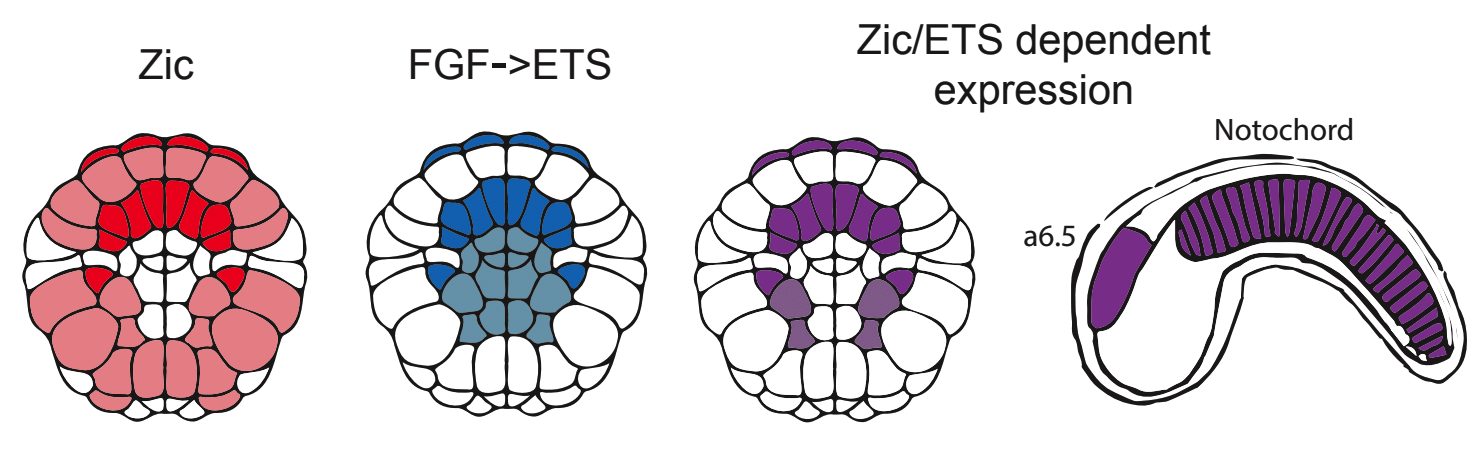
\includegraphics[scale=0.25]{1_figures-and-files/Fig1_ZicEts-Expression.png}
    \caption[Figure caption title.]{\textbf{Figure caption detailing subpanels as necessary.}}
    \label{fig:1 figure title for table of contents}
\end{figure}

%%%%%%%%%%%%%%%%%%%%%%%%%%%%%%%%%%%%%%%%%%%%%%%%%%%%%%%%%%%%%%%%%%%%%%%%%%%%%%%%
\section{Results}
%%%%%%%%%%%%%%%%%%%%%%%%%%%%%%%%%%%%%%%%%%%%%%%%%%%%%%%%%%%%%%%%%%%%%%%%%%%%%%%%

\subsection{Subsection title}

Text here.

%%%%%%%%%%%%%%%%%%%%%%%%%%%%%%%%%%%%%%%%%%%%%%%%%%%%%%%%%%%%%%%%%%%%%%%%%%%%%%%%
\section{Discussion}
%%%%%%%%%%%%%%%%%%%%%%%%%%%%%%%%%%%%%%%%%%%%%%%%%%%%%%%%%%%%%%%%%%%%%%%%%%%%%%%%

In this study \ldots

\subsection{Subsection title}

%%%%%%%%%%%%%%%%%%%%%%%%%%%%%%%%%%%%%%%%%%%%%%%%%%%%%%%%%%%%%%%%%%%%%%%%%%%%%%%%
\section{STAR*Methods}
%%%%%%%%%%%%%%%%%%%%%%%%%%%%%%%%%%%%%%%%%%%%%%%%%%%%%%%%%%%%%%%%%%%%%%%%%%%%%%%%

%%% %%% %%% %%% %%% %%% %%% %%% %%% %%% %%% %%% %%% %%% %%% %%% %%% %%% %%% %%%
\subsection{Key resources table}

\begin{landscape} % this table is long, so it'll be multi-page landscape
    \begin{longtable}{p{.49\textwidth} p{.35\textwidth} p{.5\textwidth}}
        % Define the table title in the table of contents
        \caption{Key resources table} \\ \hline 

        % Define the table columns for the first and all subsequent pages
        \multicolumn{1}{l}{\textbf{REAGENT or RESOURCE}} & \multicolumn{1}{l}{\textbf{SOURCE}} & \multicolumn{1}{l}{\textbf{IDENTIFIER}} \\ \hline \endfirsthead

        \multicolumn{3}{l}%
        {{\textbf{\tablename\ \thetable{}.} Key resources table, \textit{continued from previous page}}} \\
        \hline 
        \multicolumn{1}{l}{\textbf{REAGENT or RESOURCE}} & \multicolumn{1}{l}{\textbf{SOURCE}} & \multicolumn{1}{l}{\textbf{IDENTIFIER}} \\ \hline\hline \endhead

        % Define the table footer for the first and all subsequent pages
        \hline \multicolumn{3}{r}{\textit{Continued on next page}} \\ \hline \endfoot
        \hline \endlastfoot
        
        % Start table content

        %%%%% %%%%% %%%%% %%%%% %%%%% %%%%% %%%%% %%%%% %%%%% %%%%% %%%%% %%%%%
        \textit{Deposited Data} \\ \hline
        Data Info \\ 
        Data Info \\
        Data Info \\
        Data Info \\
        Data Info \\
        Data Info \\
        Data Info \\
        
        %%%%% %%%%% %%%%% %%%%% %%%%% %%%%% %%%%% %%%%% %%%%% %%%%% %%%%% %%%%%
        \hline \textit{Experimental Models: Organisms/Strains} \\ \hline
        \textit{Ciona} intestinalis type A (\textit{Ciona} robusta) & M-Rep & N/A \\

        %%%%% %%%%% %%%%% %%%%% %%%%% %%%%% %%%%% %%%%% %%%%% %%%%% %%%%% %%%%%
        \hline \textit{Oligonucleotides} \\ \hline
        Oligonucleotides for library screen, see Table S1 & This paper & N/A \\
        Oligonucleotides for mutagenesis, see Table S4 & This paper & N/A \\

        %%%%% %%%%% %%%%% %%%%% %%%%% %%%%% %%%%% %%%%% %%%%% %%%%% %%%%% %%%%%
        \hline \textit{Recombinant DNA} \\ \hline
        Plasmid: BraS bpFog$>$GFP & Farley Lab & N/A \\ 
        Plasmid: BraS -ZEE bpFog$>$GFP & This paper & N/A \\
        Plasmid: BraS rZE bpFog$>$GFP & This paper & N/A \\
        Plasmid: BraS -FoxA bpFog$>$GFP & This paper & N/A \\
        Plasmid: BraS -Bra bpFog$>$GFP & This paper & N/A \\ 
        Plasmid: BraS rZEFB bpFog$>$GFP & This paper & N/A \\
        Plasmid: Lama1 bpFog$>$GFP & This paper & N/A \\
        Plasmid: Lama1 bpFog$>$GFP & This paper & N/A \\
        Plasmid: Lama1 -E3 bpFog$>$GFP & This paper & N/A \\
        Plasmid: Lama1 -Z bpFog$>$GFP & This paper & N/A \\
        Plasmid: Lama1 RE3 bpFog$>$GFP & This paper & N/A \\

        %%%%% %%%%% %%%%% %%%%% %%%%% %%%%% %%%%% %%%%% %%%%% %%%%% %%%%% %%%%%
        \hline \textit{Software and Algorithms} \\ \hline
        Python (version 3.8.6)  & Python Software Foundation & \href{https://www.python.org}{https://www.python.org} \\
        Conda (version 4.9.2) & Anaconda, Inc. & \href{https://docs.conda.io/}{https://docs.conda.io} \\
        Bioconda  & Grüning et al., 2018 & \href{https://bioconda.github.io}{https://bioconda.github.io} \\
        Biopython (version 1.78) & Cock et al., 2009 & \href{https://biopython.org}{https://biopython.org} \\
        FastQC (version 0.11.9)	& Babraham Institute & \href{https://www.bioinformatics.babraham.ac.uk/}{https://www.bioinformatics.babraham.ac.uk} \\
        MultiQC (version 1.8) & Ewels et al., 2016 & \href{https://multiqc.info}{https://multiqc.info} \\
        FLASH (version 1.2.11) & Magoč et al., 2011 & \href{http://www.cbcb.umd.edu/software/flash}{http://www.cbcb.umd.edu/software/flash} \\
        \verb|pandas| (version 1.2.1) & NumFOCUS & \href{https://pandas.pydata.org}{https://pandas.pydata.org} \\
        \verb|numpy| (version 1.20.3) & Harris et al., 2020 & \href{https://numpy.org}{https://numpy.org} \\
        \verb|matplotlib| (version 3.2.2) & Hunter, 2007 & \href{https://matplotlib.org/}{https://matplotlib.org} \\
        \verb|scikit-learn| (version 0.24.1) & Pedregosa et al., 2011 & \href{https://scikit-learn.org/}{https://scikit-learn.org} \\
        \verb|seaborn| (version 0.11.1) & Waskom et al., 2021 & \href{https://seaborn.pydata.org/}{https://seaborn.pydata.org} \\
        \verb|Diverse-Logics-Notochord-Study| & Code used in this paper & \href{https://github.com/Github/RepoName}{RepoName Github} \\
    \end{longtable}
\end{landscape}

%%% %%% %%% %%% %%% %%% %%% %%% %%% %%% %%% %%% %%% %%% %%% %%% %%% %%% %%% %%%
\subsection{Resource availability}

%%% %%% %%% %%% %%% %%% %%% %%% %%% %%% %%% %%% %%% %%% %%% %%% %%% %%% %%% %%%
\subsubsection{Lead contact} 
Further information and requests for resources and reagents should be directed to and will be fulfilled by the lead contact, Professor One (\href{mailto:email@gmail.com}{email@gmail.com}). 

%%% %%% %%% %%% %%% %%% %%% %%% %%% %%% %%% %%% %%% %%% %%% %%% %%% %%% %%% %%%
\subsubsection{Materials availability} 
Plasmids generated in this study are available upon request. 

%%% %%% %%% %%% %%% %%% %%% %%% %%% %%% %%% %%% %%% %%% %%% %%% %%% %%% %%% %%%
\subsection{Experimental model and subject details}
\subsubsection{Tunicates}
Adult \textit{\textit{Ciona} intestinalis type A}, also known as \textit{\textit{Ciona} robusta}, were obtained from M-Rep and were maintained under constant illumination in seawater (obtained from Reliant Aquariums) at $18^\circ$C. \textit{Ciona} are hermaphroditic, therefore there is only one possible sex for individuals. Age or developmental stage of the embryos studied are indicated in the main text. 

%%% %%% %%% %%% %%% %%% %%% %%% %%% %%% %%% %%% %%% %%% %%% %%% %%% %%% %%% %%%
\subsection{Method details}
\subsubsection{Library Construction}
Details here.

\subsubsection{GFP reporter assays}
Details here.


%%%%%%%%%%%%%%%%%%%%%%%%%%%%%%%%%%%%%%%%%%%%%%%%%%%%%%%%%%%%%%%%%%%%%%%%%%%%%%%%
\section{Data and code availability}
%%%%%%%%%%%%%%%%%%%%%%%%%%%%%%%%%%%%%%%%%%%%%%%%%%%%%%%%%%%%%%%%%%%%%%%%%%%%%%%%

Any additional information required to reanalyze the data reported in this paper is available from the lead contact upon request. 

%%%%%%%%%%%%%%%%%%%%%%%%%%%%%%%%%%%%%%%%%%%%%%%%%%%%%%%%%%%%%%%%%%%%%%%%%%%%%%%%
\section{Acknowledgments}
%%%%%%%%%%%%%%%%%%%%%%%%%%%%%%%%%%%%%%%%%%%%%%%%%%%%%%%%%%%%%%%%%%%%%%%%%%%%%%%%

We thank \dots for helpful discussions and comments on the manuscript. This work was supported by \dots.

% Include the acknowledgement that this is a reformatted reprint
Chapter 1,  in full,  is  a  reformatted  reprint  of  the  material as it appears in “Paper title”  Author A. One, Author B. Two. \textit{Science}, 2023.  The dissertation author was the primary investigator and co-first author of this paper.

%%% %%% %%% %%% %%% %%% %%% %%% %%% %%% %%% %%% %%% %%% %%% %%% %%% %%% %%% %%%
\subsection{Author contributions}
A.A.O. designed experiments. A.A.O. and A.B.T. conducted experiments. A.A.O. analyzed data. A.A.O. and A.B.T. wrote the manuscript.

%%% %%% %%% %%% %%% %%% %%% %%% %%% %%% %%% %%% %%% %%% %%% %%% %%% %%% %%% %%%
\subsection{Declaration of interests}
The authors declare no competing interests.

\chapter{Doxorubicin-induced stress in cardiomyocytes results in RNA localization changes}\label{chap:chapter2}

\section{Introduction}

Doxorubicin (DOX) was once one of the most effective broad-spectrum anti-cancer anthracycline antibiotics\cite{kalyanaramanTeachingBasicsMechanism2020,youngAnthracyclineAntineoplasticDrugs1981} with particular efficacy against solid malignancies such as lung and breast cancer, as well as hematologic neoplasia\cite{sheibaniDoxorubicinInducedCardiotoxicityOverview2022,yuRecentProgressDoxorubicininduced2018}. However, DOX's propensity to cause cardiac damage in patients has led to significant limitations in its clinical use\cite{rahmanAnthracyclineinducedCardiotoxicityCardiacsparing2007}. There are two known mechanisms of action by which DOX acts in cells\cite{teweyAdriamycininducedDNADamage1984}: generation of reactive oxygen species via potential interactions with oxidation reaction pathways which then damage lipid membranes, disrupt mitochondrial function, induce DNA damage and triggers apoptotic pathways; and direct interaction with DNA topoisomerase II to induce single-stranded and double-stranded breaks. The exact mechanism by which DOX induces heart failure is unclear, but significant evidence suggests cardiomyocyte injury driven by oxidative stress as a major factor\cite{asensio-lopezDoxorubicininducedOxidativeStress2017,sheibaniDoxorubicinInducedCardiotoxicityOverview2022,simunekAnthracyclineinducedCardiotoxicityOverview2009,xiongProtectiveEffectBerberine2018,xuEffectsDoxorubicinMyocardium2001}. Specifically, DOX causes stress and dysfunction in multiple cellular compartments in cardiomyocytes such as mitochondria, Sarco/endoplasmic reticulum (SER), deficiencies in calcium signaling, and lipid degradation at the cellular membrane\cite{rawatDoxorubicininducedCardiotoxicityUpdate2021}. There is growing evidence that DOX not only interacts with DNA, but also with some affinity to double-stranded RNAs\cite{rubioDoxorubicinBindsDuplex2016}, rRNAs\cite{marcheschiSelectionCharacterizationSmall2009} and RNA aptamers\cite{bagalkotAptamerDoxorubicinPhysical2006}.

Having established Bento's utility to characterize RNA localization in cell lines (see Chapter \ref{chap:chapter 1}), we applied Bento to doxorubicin-treated and untreated cardiomyocytes, a cell line model for these cardiomyopathies. We performed single molecule spatial transcriptomics (Molecular Cartography) on doxorubicin-treated and untreated cardiomyocytes to measure consequential differences across multiple classes of phenotypes in a single experiment: RNA localization, gene expression, cell morphology.

\section{Results}

We designed a panel of 100 genes to profile with spatial transcriptomics, capturing pathways for cardiomyocyte health and function\cite{mahBentoToolkitSubcellular2022}. These include genes involved in cardiomyocyte contraction and conduction; cellular cytoskeletal pathways including myofibril assembly and cytoskeleton components; and also mitochondrial function to capture perturbations to oxidative metabolism. We reasoned that we could recapitulate known dysfunction of subcellular domains in cardiomyocytes upon DOX stress and measure novel RNA localization phenotypes that are not explained by expression changes alone.

\begin{figure}[p]
    \centering
    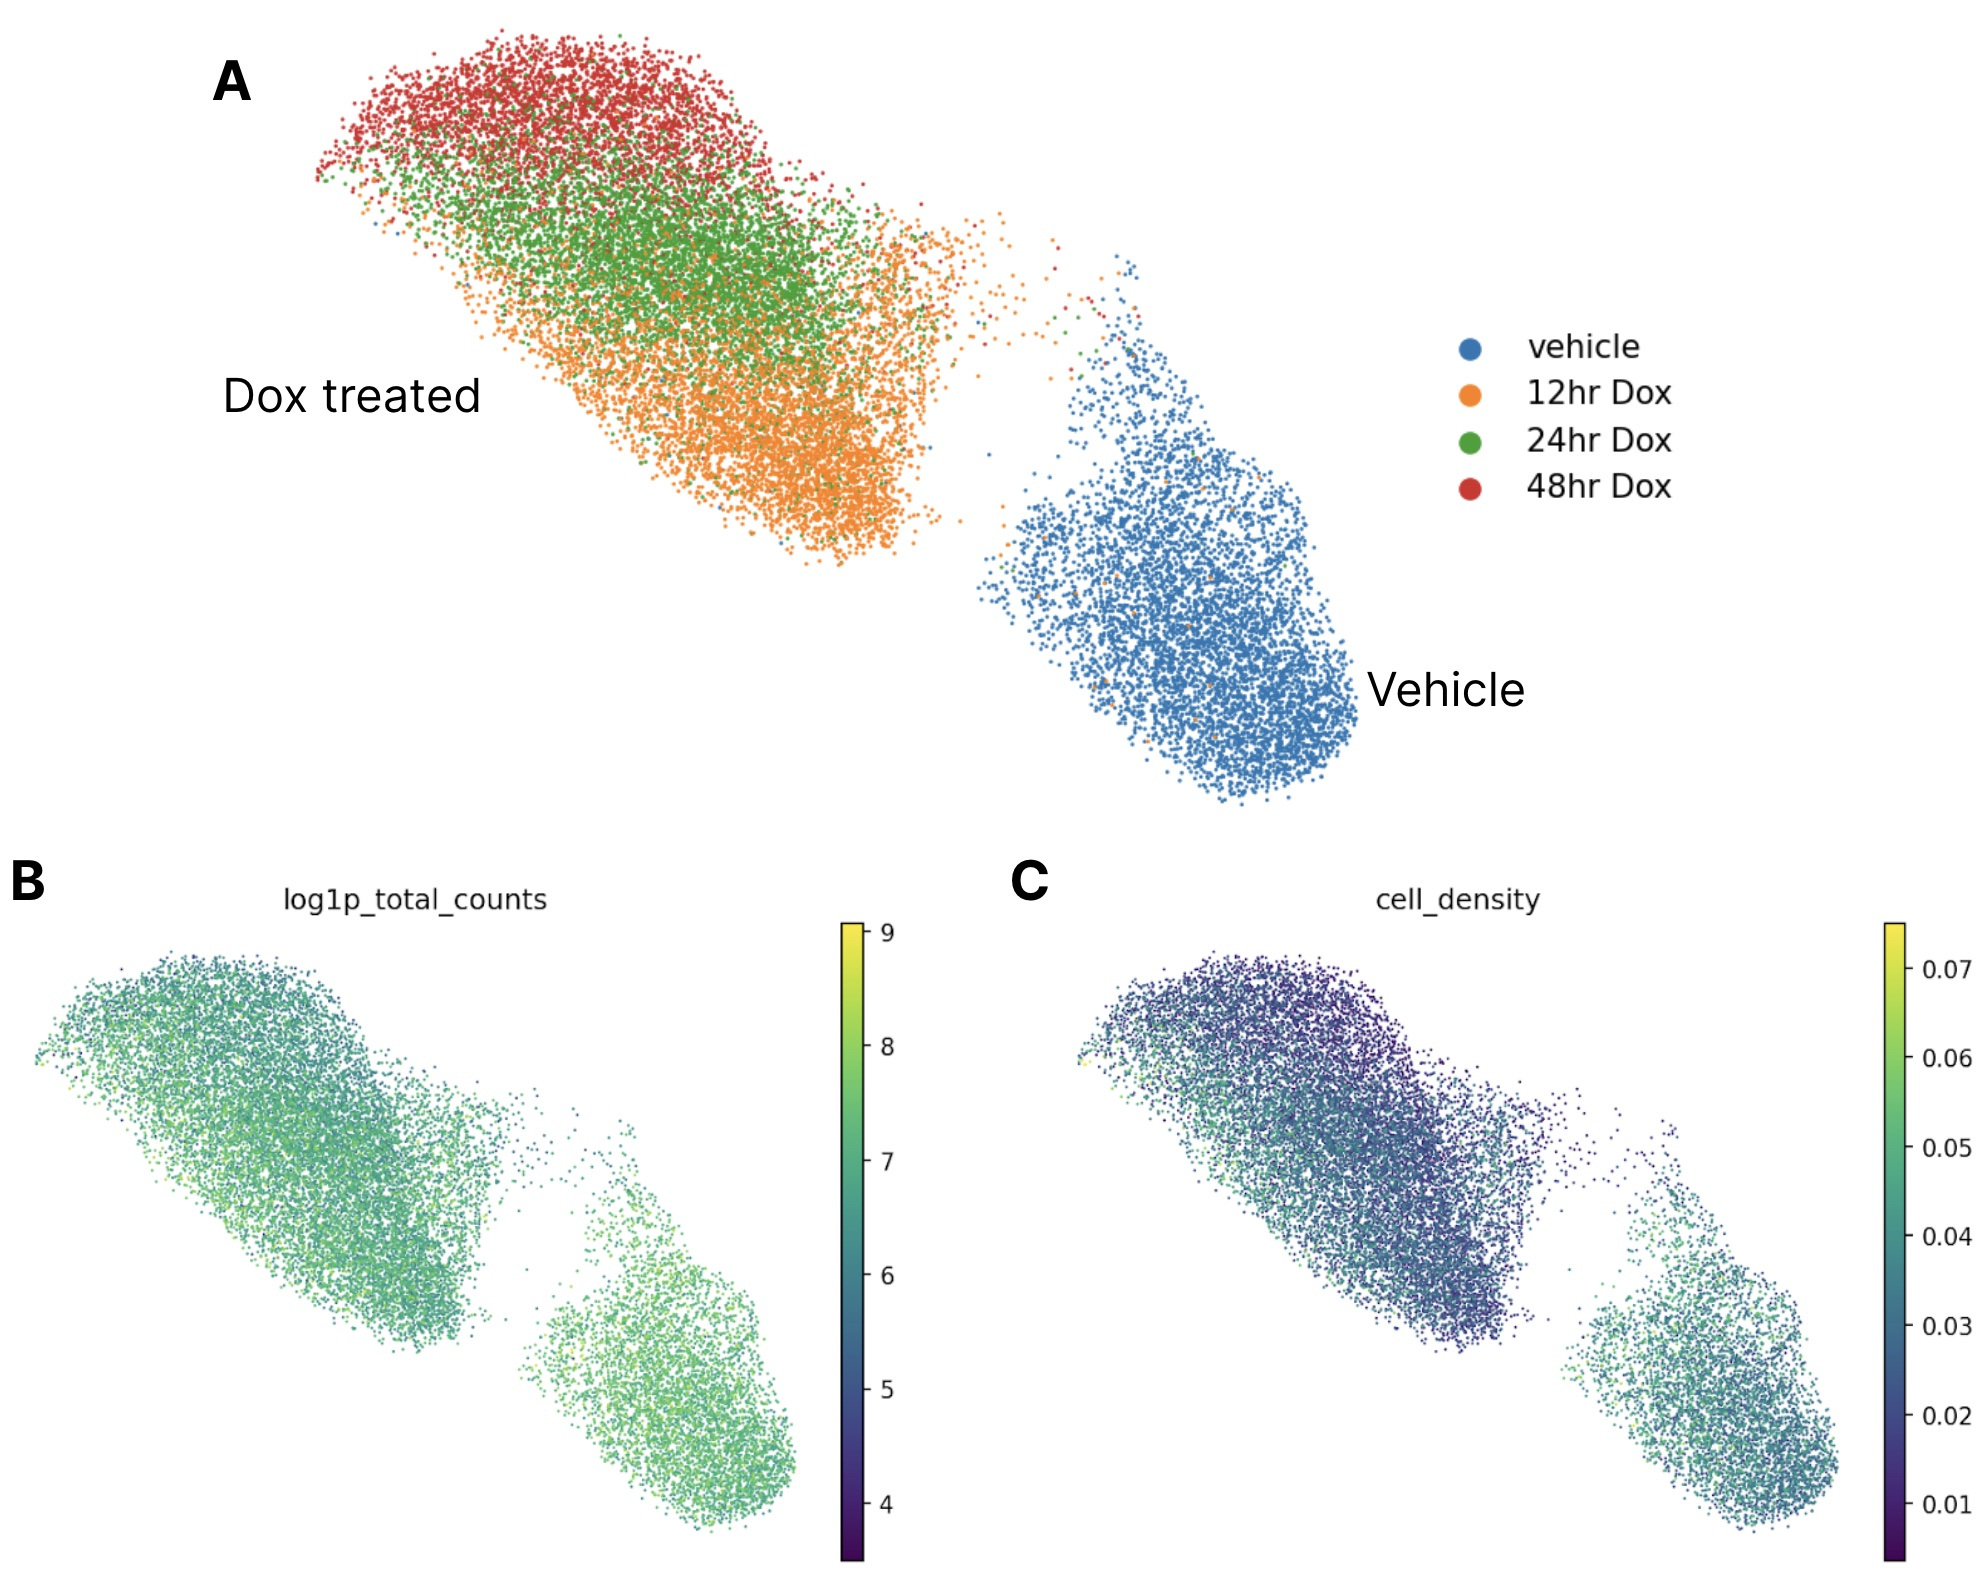
\includegraphics[width=\textwidth]{2_figures-and-files/Fig1.jpg}
    \caption[Single-cell expression of doxorubicin-treated caradiomyocytes time points]{\textbf{Single-cell expression of doxorubicin-treated caradiomyocytes time points} A. UMAP projection of single-cell expression of vehicle and doxorubicin-treated cardiomyocytes across vehicle, 12 hour, 24 hour, and 48 hour time points. Two replicates per time point. B. UMAP projection of single-cells colored by log-scaled total RNA expression and C. transcript density (transcript count divided by cell area).}
    \label{fig:Doxorubicin treatment single-cell expression}
\end{figure}

We utilized a chemically-defined protocol to differentiate human induced pluripotent stem cells (iPSCs) into beating cardiomyocytes and treated them with either DMSO (vehicle) or 2.5 uM DOX for twelve hours, 24 hours, or 48 hours before fixation (Methods). Each treatment had 2 replicates. Single molecule spatial transcriptomes were measured by Resolve Bioscience using Molecular Cartography. The resulting data was segmented using ClusterMap\cite{heClusterMapMultiscaleClustering2021} for cell boundaries and Cellpose\cite{stringerCellposeGeneralistAlgorithm2021} for nuclei boundaries. Non-myocytes were filtered out using SLC8A1 as a canonical marker for cardiomyocytes (Methods, Supp. Fig. 1A). 


Comparing vehicle and DOX treated cardiomyocytes, we found vehicles cells to cluster distinctly from all DOX treated cells (Fig. 1) and DOX treated cells forming a duration-dependent expression gradient from 12-48 hours. Notably, transcript density i.e. transcript count dividedby cell area, decreases with treatment duration. Differential expression analysis of each timepoint relative to vehicle indicate that DOX induces cellular stress as expected. NPPA and NPPB are important biomarkers in clinical cardiology that become upregulated during cardiac stress\cite{manStructureFunctionNppa2018,songAtrialNatriureticPeptide2015}. Elevated levels of NPPB have been used to diagnose patients with doxorubicin induced cardiotoxicity and elevated levels of NPPB also correlate with severity of heart failure. An increase in NPPA and NPPB levels upon Doxorubicin exposure at 24 and 48 hours indicates that the cardiomyocytes have transitioned to a state of cellular stress (Fig. 2A,B).

We then restricted our analysis to focus on the 12 hour treatment and vehicle for spatial analyses via Bento. Poor segmentation quality for the other timepoints limited the precision and accuracy of 2-dimensional spatial analysis algorithms. We identified subcellular domains in vehicle and 12 hour DOX treated cardiomyocytes using RNAflux, clustering the domains into four fluxmap domains (Fig. 2C). Enrichment of location-specific gene expression aligned domains to the nucleus (nuclear pore, nucleolus, and nucleus), ERM and OMM, ER lumen, and cytosol respectively (Fig. 2C \& D, Supp. Fig. 1C). Comparing the gene composition in each domain, we observe an overall localization bias towards both the nucleus and ERM/OMM in vehicle treated cells (**Fig. 2E top**), in agreement to prior poly(A) smFISH studies\cite{lewisLocalizationTranscriptsTranslation2018}. However, RNA in the DOX treated cardiomyocytes demonstrated a shift in average RNA localization away from the ERM/OMM and towards the nucleus (**Fig. 2C bottom**). There is evidence that 90\% of genes have a half life of less than 260 minutes\cite{smalecGenomewideQuantificationRNA2022}, far less than the 12 hour DOX treatment, indicating that the shift in RNA localization is likely due to reduced nuclear export of newly synthesized RNA from the nucleus to the ERM/OMM. Indeed, even low concentrations of DOX have been demonstrated to alter structural fibrous proteins as well as mitochondrial depolarization and fragmentation\cite{sardaoMorphologicalAlterationsInduced2009}. Of particular note, the RNA binding protein RBM20 – a critical regulator of mRNA splicing of genes encoding key structural proteins associated with cardiac development and function – had a pronounced depletion of RNA transcripts outside of the nucleus upon DOX treatment (Fig. 2F). With further validation, this may indicate nuclear retention and or degradation of nuclear exported RBM20 mRNA as a potential mechanism of DOX induced cardiomyopathy. Similarly, we found the mRNA of calcium voltage-gated channel subunit CACNB2 to also deplete outside of the nucleus (Fig. 2G). The loss of CACNB2 translation outside of the nucleus may impact calcium signaling crucial to cardiomyocyte function\cite{meissnerModerateCalciumChannel2011}.

\begin{figure}[p]
    \centering
    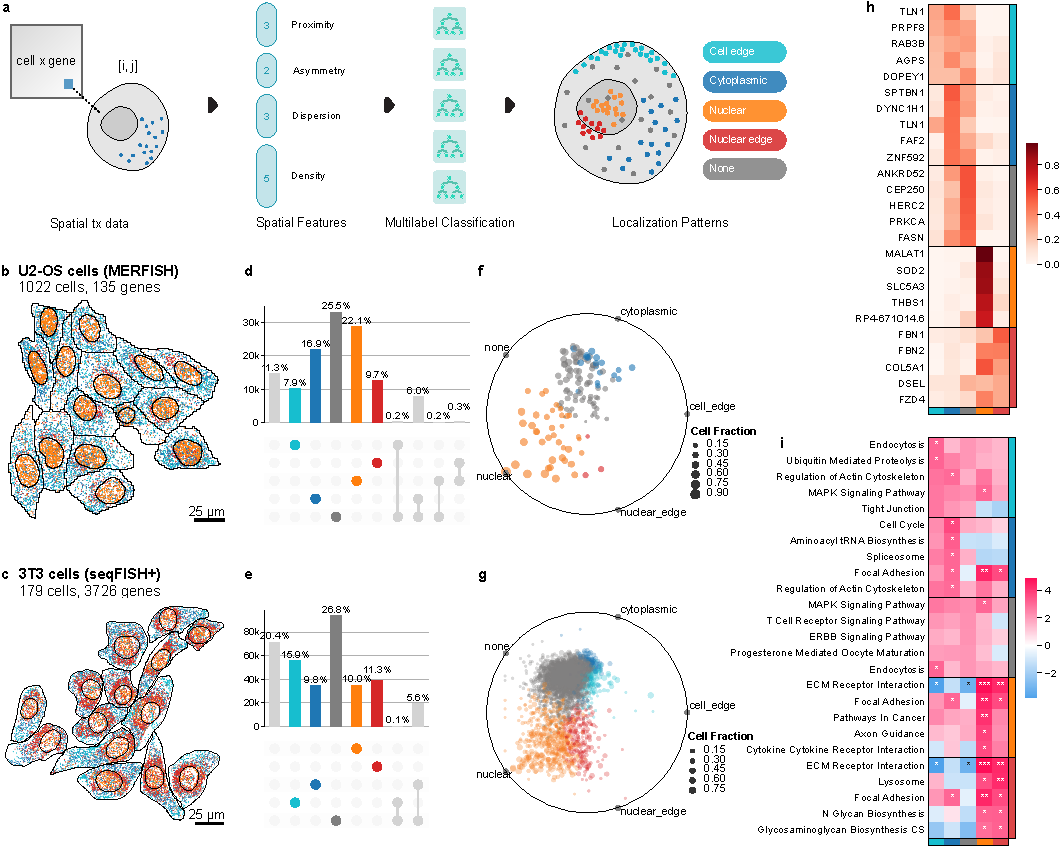
\includegraphics[width=\textwidth]{2_figures-and-files/Fig2.pdf}
    \caption[Subcellular RNA localization changes upon Doxorubicin treatment in iPSC-derived cardiomyocytes]{\textbf{Subcellular RNA localization changes upon Doxorubicin treatment in iPSC-derived cardiomyocytes} A. Cardiomyocytes derived from human iPSCs were treated with DMSO or 2.5 uM DOX for 12 hours. The localizations of 100 genes relevant to cardiomyocyte health and function were measured using Molecular Cartography. Cell boundaries were determined using ClusterMap and nuclei were segmented using Cellpose. B. Top 10 upregulated and downregulated genes in vehicle versus treatment. C. APEX-seq location-specific gene enrichment of fluxmap domains for the cytosol, endoplasmic reticulum membrane (ERM), endoplasmic reticulum lumen (ER Lumen), nuclear lamina, nucleus, nucleolus, nuclear pore and outer mitochondrial matrix (OMM). D. Fluxmap domains visualized for a representative field of view of cardiomyocytes for vehicle and treatment respectively highlighting cellular nuclei, ERM/OMM, ER Lumen, and cytosol. E. RNAflux fluxmap enrichment of each gene averaged across vehicle and treatment cardiomyocytes captures changes in subcellular RNA localization. Visualization of RBM20 F. and CACNB2 G. confirms the depletion of transcripts from the perinuclear and cytosolic compartments of cardiomyocytes upon DOX treatment.}
    \label{fig:Doxorubicin treatment cardiomyocytes}
\end{figure}

\section{Discussion}

In this study of DOX-induced stress in cardiomyocytes, we utilized single-molecule spatial transcriptomics to identify changes in both gene expression and subcellular RNA localization resulting from DOX treatment. Of particular interest was the RNA binding protein RBM20, whose extranuclear depletion in mRNA represents a potential target for therapeutic intervention. This localization behavior may be an early consequence leading to the functional mis-splicing of RBM20's cardiomyopathy-associated targets. Sequestration of the mRNA may be an indirect mechanism of down-regulation. The ERM-associated fluxmap seems to be relatively larger in DOX treated cells compared to vehicle, suggesting that remodeling of organelles may drive movement of molecules or vice versa. 

We found that the 2D spatial resolution of molecular coordinates and segmentation data to limit the clarity of our analyses. While the Clustermap based cell segmentation was sufficient to approximate subcellular domains with RNAflux in the vehicle and 12 hour treatment samples, many regions of the 24 hour and 48 hour treatment samples have denser cells that sit on top of one another due to tighter cell seeding densities. As a result, molecular coordinates and segmentations were flattened to two dimensions, making it impossible to disambiguate expression patterns from overlapping cells. We foresee that better resolution and 3D compatible segmentation algorithms will alleviate this in the future. This is likely required for analysis to achieve subcellular resolution in more complex systems e.g. tissue slices and organoids.

Due to the targeted nature of the particular spatial transcriptomics platform, the 100 gene panel is biased for genes annotated for cardiac function, limiting discovery of novel targets. Expanding the panel size would allow us to capture a better picture of spatial perturbations to the transcriptomic landscape. Additionally, generalizing spatial analyses in Bento from 2D to 3D would enable finer segmentation of subcellular compartments and cells, in turn improving RNA localization analysis. Overcoming these challenges will be useful not only for enabling spatial analysis to other cell lines and conditions, but also to even more heterogeneous systems such as tissue.

\section{Methods}

\subsection{Preprocessing cardiomyocytes datasets}
Single-cell expression matrices of both vehicle replicates and both DOX treatment samples were concatenated as a single expression matrix. Cells were projected into two dimensions with UMAP dimensional reduction. No significant batch effects were detected. Leiden clustering was performed at resolution=0.5 to isolate and filter out a non-myocyte population depleted in SLC8A1 expression (Supp. Fig. 1A). All described preprocessing steps were performed in Scanpy\cite{wolfSCANPYLargescaleSinglecell2018}.

\subsection{RNAflux: Unsupervised spatial embedding and subcellular domain quantization}

For the iPSC-derived cardiomyocytes, a step size of 5 data units was used to compute RNAflux embeddings. Visualization and enrichment of locale-specific transcriptomes derived by APEX-seq were performed as described in Chapter \ref{chap:chapter 1}.

\subsection{Molecular Cartography}
\textit{Cultured cell processing.} After Doxorubicin treatment, cardiomyocytes were washed with PBS (1x) twice and fixed in Methanol (-20°C) for 10 min. After fixation, Methanol was aspirated and cells were dried and stored at -80°C until use. The samples were used for Molecular CartographyTM (100-plex combinatorial single molecule fluorescence in-situ hybridization) according to the manufacturer’s instructions Day 1: Molecular Preparation Protocol for cells,  starting with the addition of buffer DST1  followed by cell priming and hybridization. Briefly, cells were primed for 30 minutes at 37°C followed by overnight hybridization of all probes specific for the target genes (see below for probe design details and target list). Samples were washed the next day to remove excess probes and fluorescently tagged in a two-step color development process. Regions of interest were imaged as described below and fluorescent signals removed during decolorization. Color development, imaging and decolorization were repeated for multiple cycles to build a unique combinatorial code for every target gene that was derived from raw images as described below.
Probe Design. The probes for 100 genes were designed using Resolve's proprietary design algorithm. Briefly, the probe-design was performed at the gene-level. For every targeted gene, all full-length protein coding transcript sequences from the ENSEMBL database were used as design targets if the isoform had the GENCODE annotation tag `basic'\cite{frankishGENCODEReferenceAnnotation2019,yatesEnsembl20202019}. To speed up the process, the calculation of computationally expensive parts, especially the off-target searches, the selection of probe sequences was not performed randomly, but limited to sequences with high success rates. To filter highly repetitive regions, the abundance of k-mers was obtained from the background transcriptome using Jellyfish\cite{marcaisFastLockfreeApproach2011}. Every target sequence was scanned once for all k-mers, and those regions with rare k-mers were preferred as seeds for full probe design. A probe candidate was generated by extending a seed sequence until a certain target stability was reached. A set of simple rules was applied to discard sequences that were found experimentally to cause problems. After these fast screens, the remaining probe candidates were mapped to the background transcriptome using ThermonucleotideBLAST\cite{gansImprovedAssaydependentSearching2008} and probes with stable off-target hits were discarded. Specific probes were then scored based on the number of on-target matches (isoforms), which were weighted by their associated APPRIS level\cite{rodriguezAPPRIS2017Principal2018}, favoring principal isoforms over others. A bonus was added if the binding-site was inside the protein-coding region. From the pool of accepted probes, the final set was composed by picking the highest scoring probes. Probes with catalog numbers can be found in Supp. Table 1\cite{mahBentoToolkitSubcellular2022}. 

\textit{Imaging.} Samples were imaged on a Zeiss Celldiscoverer 7, using the 50x Plan Apochromat water immersion objective with an NA of 1.2 and the 0.5x magnification changer, resulting in a 25x final magnification. Standard CD7 LED excitation light source, filters, and dichroic mirrors were used together with customized emission filters optimized for detecting specific signals. Excitation time per image was 1000 ms for each channel (DAPI was 20 ms). A z-stack was taken at each region with a distance per z-slice according to the Nyquist-Shannon sampling theorem. The custom CD7 CMOS camera (Zeiss Axiocam Mono 712, 3.45 um pixel size) was used. For each region, a z-stack per fluorescent color (two colors) was imaged per imaging round. A total of 8 imaging rounds were done for each position, resulting in 16 z-stacks per region. The completely automated imaging process per round was realized by a custom python script using the scripting API of the Zeiss ZEN software (Open application development).

\textit{Image Processing and Spot Segmentation.} As a first step all images were corrected for background fluorescence. A target value for the allowed number of maxima was determined based upon the area of the slice in um² multiplied by the factor 0.5. This factor was empirically optimized. The brightest maxima per plane were determined, based upon an empirically optimized threshold. The number and location of the respective maxima was stored. This procedure was done for every image slice independently. Maxima that did not have a neighboring maximum in an adjacent slice (called z-group) were excluded. The resulting maxima list was further filtered in an iterative loop by adjusting the allowed thresholds for (Babs-Bback) and (Bperi-Bback) to reach a feature target value (Babs: absolute brightness, Bback: local background, Bperi: background of periphery within 1 pixel). This feature target values were based upon the volume of the 3D-image. Only maxima still in a zgroup of at least 2 after filtering were passing the filter step. Each z-group was counted as one hit. The members of the z-groups with the highest absolute brightness were used as features and written to a file. They resemble a 3D-point cloud. To align the raw data images from different imaging rounds, images had to be registered. To do so the extracted feature point clouds were used to find the transformation matrices. For this purpose, an iterative closest point cloud algorithm was used to minimize the error between two point-clouds. The point clouds of each round were aligned to the point cloud of round one (reference point cloud). The corresponding point clouds were stored for downstream processes. Based upon the transformation matrices the corresponding images were processed by a rigid transformation using trilinear interpolation. The aligned images were used to create a profile for each pixel consisting of 16 values (16 images from two color channels in 8 imaging rounds). The pixel profiles were filtered for variance from zero normalized by total brightness of all pixels in the profile. Matched pixel profiles with the highest score were assigned as an ID to the pixel. Pixels with neighbors having the same ID were grouped. The pixel groups were filtered by group size, number of direct adjacent pixels in group, number of dimensions with size of two pixels. The local 3D-maxima of the groups were determined as potential final transcript locations. Maxima were filtered by the number of maxima in the raw data images where a maximum was expected. Remaining maxima were further evaluated by the fit to the corresponding code. The remaining maxima were written to the results file and considered to resemble transcripts of the corresponding gene. The ratio of signals matching to codes used in the experiment and signals matching to codes not used in the experiment were used as estimation for specificity (false positives). The algorithms for spot segmentation were written in Java and are based on the ImageJ library functionalities. Only the iterative closest point algorithm is written in C++ based on the libpointmatcher library (https://github.com/ethz-asl/libpointmatcher).

\textit{Image segmentation.} Cellpose v1.0.2\cite{stringerCellposeGeneralistAlgorithm2021} was used to perform image segmentation to determine the boundaries of nuclei. The nuclei boundaries were determined by running Cellpose with the `nuclei' model using default parameters on the DAPI stain channel of the pre-hybridization images. Cytoplasm boundaries were determined with ClusterMap\cite{heClusterMapMultiscaleClustering2021} using spot coordinates.

\subsection{iPSC Cardiac Differentiation and Doxorubicin Treatment}
Matrigel (Corning, cat \# 354277) coated plates were used to culture iPSCs with mTESR Plus human iPSC medium (StemCell Technologies, cat \# 100-0276) in a humidified incubator at 37°C with 5\% CO2. iPSCs were dissociated with Gentle Cell Dissociation Reagent (StemCell Technologies, cat \# 100-0485) and passaged with mTESR Plus medium and 10uM ROCK inhibitor (Tocris, cat \#1254) at a ratio of 1:12. mTESR plus medium was replaced every other day until the cells reached 80\% confluency for maintenance and replating, or 90\% confluency for cardiac differentiation utilizing a chemically defined protocol\cite{lianRobustCardiomyocyteDifferentiation2012}. On day 0 of cardiac differentiation, cells were treated with 6uM CHIR99021 (Selleck Chem, cat \# S1263) in RPMI 1640 media (Gibco, cat \# 11875) and B27 minus insulin supplement (Thermo Fisher, cat \# A1895601). On day 2, CHIR was removed, and cells were cultured with RPMI 1640 media and B27 minus insulin supplement (Thermo Fisher, cat \# A18956). On day 3, media was replaced with RPMI media containing B27 minus insulin supplement and 5 uM Wnt-C59 (Cellagen Technologies, cat \# C7641-2s). On days 5, 7, and 9, media was replaced with RPMI media containing B27 insulin supplement (Thermo Fisher, cat \# 17504). On days 11 and 13, media was replaced with RPMI 1640 media without glucose (Thermo Fisher, cat \# 11879020) containing B27 insulin supplement for purification of cardiomyocytes. From days 15 onward, the cells were cultured in RPMI 1640 media containing B27 supplement which was changed every other day until the cells reached day 30 for replating. For replating, cells were incubated in 10X TrypLE (Thermo Fisher, cat \# A1217701) for 12 minutes at 37 C, neutralized with equal volumes of RPMI 1640 media containing B27 supplement with 20\% FBS (Gibco, cat \# 26140-079), gently dissociated by pipetting, then spun down and resuspended for replating in RPMI 1640 media containing B27 supplement with 20\% FBS. The next day, the cell media was replaced with RPMI 1640 media containing B27 supplement which was replaced with fresh media every other day. On day 48 the cells were replated onto chamber slides (Ibidi, cat \# 80826) as described above and recovered for 10 days before doxorubicin treatments began (MedChemExpress, cat \# HY-15142). On day 60, doxorubicin treatments concluded, and the cells underwent methanol fixation.

\subsection{Data Availability}
Preprocessed data for Molecular Cartography profiled cardiomyocytes is deposited at https://doi.org/10.6084/m9.figshare.c.6564043.v1 and is accessible through the Bento Python package. 

\subsection{Code Availability}
Analysis code for generating figures can be found at: https://github.com/ckmah/bento-manuscript.

\subsection{Acknowledgements}

As this work was derived from the same manuscript, see \ref{chap:chapter 1} for corresponding details.

\subsection{Author Contributions}
As this work was derived from the same manuscript, see \ref{chap:chapter 1} for corresponding details.

\subsection{Competing Interests}
As this work was derived from the same manuscript, see \ref{chap:chapter 1} for corresponding details.
\chapter{Spotfish: A modular framework for decoding spatial imaging data}\label{chap:chapter 3}


\section{Background}

Image-based spatial transcriptomics is a rapidly evolving field that seeks to map the spatial distribution of RNA molecules in situ. These technologies have enabled researchers to study the spatial organization of cells and tissues at unprecedented resolution, with the potential to uncover novel biological insights.The field has seen a surge in interest in recent years, with the development of several novel technologies, including MERFISH\cite{chenSpatiallyResolvedHighly2015}, seqFISH\cite{shahSeqFISHAccuratelyDetects2017}, STARmap\cite{wangThreedimensionalIntacttissueSequencing2018}, ISS\cite{keSituSequencingRNA2013}, and Slide-seq\cite{rodriquesSlideseqScalableTechnology2019}. Despite their varied underlying technologies, they consistently share the same backbone with a unified objective: reporting the location and identity of individual RNA molecules. A significant challenge in this domain is the difficulty in validating the quality of image analysis outputs. This issue is confounded by the lack of standardized data quality metrics accepted by researchers. While existing pipeline development tools for spatial transcriptomics image analysis are functional, they often suffer from limited scalability, a lack of interoperability with newer methodologies, and restricted portability across different computing environments. Recognizing these limitations, there emerges a clear need for an unbiased framework to build spatial transcriptomics pipelines. 

To address these challenges, I developed spotfish, a modular pipeline building framework that abstracts the series of tasks for processing spatial transcriptomics data by standardizing inputs and outputs between workflow tasks. This allows swapping in new tools as new alternatives are published frequently, by wrapping the chosen tool for compatible data formats. It also encourages reporting quality metrics for diagnosing data quality and evaluating the performance of chosen tool/parameter combinations. The framework is built using Nextflow, a robust workflow language specifically built for and heavily adopted by bioinformatics researchers\cite{ditommasoNextflowEnablesReproducible2017}. Nextflow also abstracts how the pipelines are executed on different computing environments, e.g. locally, on compute clusters, or various cloud services, meaning spotfish is inherently usable for researchers regardless of computational environment. In contrast to starfish's approach to programmatic Python-based pipeline construction, spotfish modules are programming language agnostic through the use of containerization for each step of the process. Additionally, the pipeline prioritizes usage of open file formats supported by the Open Microscopy Environment\cite{goldbergOpenMicroscopyEnvironment2005} (OME) to ensure transparency and compatibility with the rich ecosystem of bio-imaging analysis tools. Spotfish is guided by FAIR principles\cite{wilkinsonFAIRGuidingPrinciples2016} and utilize modern open-source standards, ensuring accessibility for a broad spectrum of users, from researchers and core facilities to technologists.

\section{Properties of multiplexed transcriptomics imaging data}

The raw data consists of a large mosaic of microscopy images. To resolve individual fluorescent molecules, images are taken at roughly to 10-100 times magnification. A single image, or field of view, contains roughly 1-100 cells depending on the magnification and cell type. The same field of view is then imaged multiple times, in which the spectrum of light is limited to specific frequency bands at each iteration. This allows us to assign a unique combination of fluorescent probes that emit light at unique frequency bands to each target. The focal plane is much narrower than the height of cells as a consequence of the high magnification, which requires imaging the same field of view multiple times at different z-planes to maximize the volume interrogated. This process is usually repeated for a grid of positions to capture a larger cumulative area of the sample, which can produce upwards of a terabyte of data per experiment. The challenge arises due to the multi-dimensional nature of these measurements, across spatial dimensions x, y and z, channels (multiple laser wavelengths), and rounds (repeated imaging with different combinations of probes).

\section{Framework Design}

Imaging-based acquisition of spatial transcriptomics data requires coordinating a series of tasks, including image stitching, registration, background correction, spot detection, and finally barcode decoding to produce labeled molecular coordinates corresponding to a predesigned set of gene targets. Every task can be accomplished with existing tools, but it remains difficult to perform an end-to-end analysis outside of tailored pipelines without significant data wrangling. Even though many studies utilize commercial platforms for spatial transcriptomics, only processed data is usually available to the customer. Their analysis pipelines remains proprietary and blackbox, forcing users to rely on arbitrarily defined quality metrics. In contrast, starfish is a open-source unified pipeline framework implemented in Python, abstracting processing steps using a object-oriented programming design\cite{othersStarfishOpenSource}. It is extremely flexible and has accommodated data processing for 7 different technologies. However, the API's steep learning curve, many parameters, and lack of maintenance makes it difficult to build pipelines and integrate cutting-edge tools without significant refactoring of the tool or starfish itself. There has only been one prominent third-party contribution by a recent development that integrated their novel barcode decoding algorithm, CheckAll\cite{cisarUnifiedPipelineFISH2023}.

Spotfish abstracts pipelines into two subworkflows: image registration and spot analysis. Image registration is a common image processing step not unique to spatial transcriptomics and is usually required for acquisitions across multiple fields of view. By decoupling this step, it is convenient to adapt tools outside of the immediate domain. The spot analysis subworkflow encompasses two tasks, spot detection and barcode decoding to produce molecular coordinate tables with target i.e. gene annotations. This can then be combined with cell and nuclear segmentation data for functional analysis in other software, such as Bento\cite{mahBentoToolkitSubcellular2022}, Squidpy\cite{pallaSquidpyScalableFramework2021} and Scanpy\cite{wolfSCANPYLargescaleSinglecell2018}.

\begin{figure}[h]
    \centering
    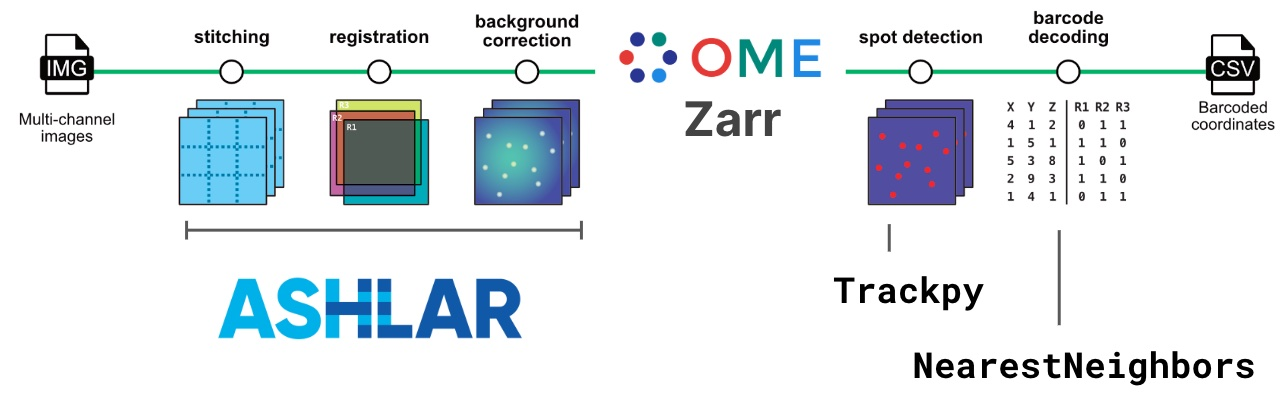
\includegraphics[width=\textwidth]{3_figures-and-files/image processing workflow.jpg}
    \caption[Spotfish workflow]{\textbf{Spotfish workflow} Overview of the analysis tasks in the spotfish workflow from left to right. Image registration encompasses stitching, registration and background correction (as needed). Intermediate output format of OME-ZARR. Spot analysis encompasses spot detection and barcode decoding outputing coordinate tables with annotations. Tools used to implement each subworkflow indicated below.}\label{fig:spotfish workflow}
\end{figure}


\section{Case Study: 69-bit MERFISH of U2-OS Cells}

To demonstrate the utility of spotfish, I applied it to previously published 69-bit MERFISH dataset of U2-OS cells designed to target 10,000 genes with a minimum hamming distance 4 (HD4) encoding scheme\cite{xiaSpatialTranscriptomeProfiling2019}. Because the experiment had a total of 72 rounds of imaging, it was suitable for testing the scalability of the the spotfish framework. Commercial platforms reportedly use 16 rounds (CosMx\cite{heHighplexMultiomicAnalysis2021}) and 15 rounds (Xenium\cite{janesickHighResolutionMapping2022}) to decode 980 and 313 targets respectively. This meant the 10k MERFISH dataset uses roughly 4.5 times more imaging rounds than the current largest commercial platforms. The specific tools implemented in the pipeline were chosen based on their performance on the 10k MERFISH dataset. The image registration step was performed using Ashlar\cite{muhlichStitchingRegisteringHighly2022}, a software package originally designed for stitching and aligning multiplexed immunofluorescent samples acquired via cyclical imaging and tile-scanning. The spot detection step was performed using trackpy\cite{SoftmatterTrackpyV0}, a Python library for particle tracking in 2D and 3D. The barcode decoding step was performed using the nearest neighbor approach implemented in the scikit-learn analysis package\cite{pedregosaScikitlearnMachineLearning2011}.

Spotfish allowed parallelization of the image registration step across all 69 rounds with Ashlar. This step was ultimately limited by memory not computing speed, using 30 GB to stitch each round in 16 cpu hours. The output of the image registration step was a 1.5 TB OME-ZARR file storing a multi-scale representation of the image data registered to the same coordinate system.  By standardizing the output format, this eliminates the need for storing additional metadata defining tile positions and channel orders. The spot detection step was performed using trackpy, which was able to detect 477 million spot coordinates in 3 dimensions. The barcode decoding step was performed using the nearest neighbor approach implemented in the scikit-learn analysis package.  Without spotfish, the total compute time is estimated to be 1248 hours whereas parallelization reduced runtime over 26-fold, to 39 hours with 32 parallel processes for spot detection and 8 parallel processes for spot calling. The output was then visualized using Napari\cite{NapariMultidimensionalImage} to assess the quality of the data interactively.

\section{Conclusion}

All together, I demonstrate spotfish's flexibility in integrating heterogeneous set of tools to build a scalable image analysis pipeline for spatial transcriptomics. By adhering to open file formats and containerization, spotfish addresses existing technologies and is well positioned to adapt to future advancements for image registration, spot detection and barcode decoding. Future work will focus on creating quality control modules that provide quantitative metrics for assessing the quality of the data at each step of the pipeline. This will allow researchers to identify the optimal tool and parameter combinations for their data. To facilitate open discussion of spotfish's development, I aim to collaborate with the nf-core community, a consortium of bioinformatics researchers that develop and maintain a collection of high quality modular bioinformatics pipelines. This will ensure that spotfish is well maintained and accessible to the community. Finally, I will continue to develop spotfish to support additional spatial transcriptomics technologies, such as seqFISH and STARmap. This will allow researchers to compare the performance of different technologies on the same dataset, and to integrate data from different technologies for meta-analysis.
\begin{dissertationepilogue}

    % Fix a bug in the numbering of the epilogue chapters?
    \setcounter{chapter}{4}
    \setcounter{section}{0}

    \section{Conclusion}

    In this dissertation, I have presented a series of computational methods to analyze spatial transcriptomics data. I began by developing Bento, a computational framework for subcellular analysis of spatial transcriptomics data. This work is one of the first to leverage the spatial resolution of imaging-based spatial transcriptomics data to study subcellular RNA localization. I demonstrated the utility of Bento by applying it to a variety of spatial transcriptomics datasets, including cardiomyocytes to study changes in RNA localization as scale. Unexpectedly, we found several genes mislocalized to the nucleus as a result of doxorubicin treatment, including RBM20 and CACNB2, suggesting that RNA localization is an underappreciated cell phenotype that has the potential to uncover functional biology. To lower the barrier to functional analysis of spatial transcriptomics datasets, I also created spotfish, a modular framework for decoding spatial imaging data. This framework is designed to be flexible, scalable, and interoperable with existing tools. I demonstrated the utility of spotfish by applying it to a 69-bit MERFISH dataset of U2-OS cells. The framework is aimed to be a community resource for building spatial transcriptomics pipelines, and I hope to eventually collaborate with the nf-core community to ensure that spotfish is well maintained and accessible to the community. 

    %%%%%%%%%%%%%%%%%%%%%%%%%%%%%%%%%%%%%%%%%%%%%%%%%%%%%%%%%%%%%%%%%%%%%%%%%%%%
    \section{Limitations and Future Directions}
    %%%%%%%%%%%%%%%%%%%%%%%%%%%%%%%%%%%%%%%%%%%%%%%%%%%%%%%%%%%%%%%%%%%%%%%%%%%%

    There are a great deal of challenges with the current generation of spatial transcriptomics data. During my graduate work, it was important to me that I focus on core problems that reveal fundamental biology, not a transient technical property of any one technology. For example, the most popular commercial spatial methods are slide-based capture assays paired with traditional sequencing for comprehensive transcriptome profiling. However, compared to imaging-based approaches which have single-molecule resolution, each spatial location on the assay captures several to tens of cells depending on the technology. This loss in fidelity has spawned an entire subfield of deconvolution methods, specifically to estimate properties of each spatial location such as the proportion of cell types, the expression of cells given predicted cell types, technical dropout of expression, etc. These techniques may be useful now, but are ultimately tied to a specific iteration of rapidly evolving spatial transcriptomic technologies. Instead, I chose to tackle problems initially hampered by the lack of tangible datasets; the recent availability of public datasets has indeed lowered the barrier to method development. The increasing throughput of new technologies such as Xenium from 10x Genomics and STOmics from BGI Genomics will only improve our ability to draw biological insights at the molecular resolution. Similarly, the imminent move towards multi-omics spatial imaging will enable us to capture more snapshots of the RNA life cycle than ever before.
    
    While the current functionality of Bento is limited to 2-dimensional spatial analysis, the obvious extension to 3 dimensions will enable subcellular analysis in biological systems more complex than monolayer cell cultures such as tissue slices and organoids. This will also open the door to exploring true physical molecular gradients in their natural 3 dimensions. While we showed its value to discover spatial subcellular domains, one can imagine gradient shifts between cells e.g. at the cell membrane, tight junctions, synapses etc. or even in the extracellular matrix characterizing cell signaling molecules. These are some of the functional biology questions waiting to be explored with spatial transcriptomics data. Bento is also capable of measuring morphological phenotypes; paired with the appropriate experimental design, spatial transcriptomics will be a powerful tool to interrogate the relationship between cell states, RNA localization, and cell morphology. These are especially relevant in developmental biology, neurological diseases, and cancer where changes to cell shapes and molecular condensates are frequently measured already. Algorithmic improvements will also require computational scalability, which I hope to address by interfacing with the global research community, including the Scverse Foundation\cite{virshupScverseProjectProvides2023} developers and the nf-core project members. Looking forward, this will manifest as integration with new open-source data standards, such as SpatialData and distributed computing with Dask. 
    

    %%%%%%%%%%%%%%%%%%%%%%%%%%%%%%%%%%%%%%%%%%%%%%%%%%%%%%%%%%%%%%%%%%%%%%%%%%%%
    \section{Closing thoughts}
    %%%%%%%%%%%%%%%%%%%%%%%%%%%%%%%%%%%%%%%%%%%%%%%%%%%%%%%%%%%%%%%%%%%%%%%%%%%%

    The field of spatial transcriptomics is still in its infancy, and there are many exciting opportunities for future computational work. I believe the most impactful innovations will come from other fields, such as computer vision and genomics. Deep learning has already made its mark in both fields to accomplish everything from self-driving cars to functional genomics with DNA large language models, with the potential to bridge the gap between imaging and sequencing. I am hopeful for the creativity in this field and am excited to see new applications beyond tissue atlases and drug screening platforms. I hope that my work will contribute to the growing body of open-source tools and resources for spatial transcriptomics, and that it will inspire others to do the same.

\end{dissertationepilogue}

%%%%%%%%%%%%%%%%%%%%%%%%%%%%%%%%%%%%%%%%%%%%%%%%%%%%%%%%%%%%%%%%%%%%%%%%%%%%%%%%
% Appendix of the Dissertation
%%%%%%%%%%%%%%%%%%%%%%%%%%%%%%%%%%%%%%%%%%%%%%%%%%%%%%%%%%%%%%%%%%%%%%%%%%%%%%%%
\appendix

\appendix{}

\chapter{Supplemental Material for Chapter \ref{chap:Title of first chapter}}

%%%%%%%%%%%%%%%%%%%%%%%%%%%%%%%%%%%%%%%%%%%%%%%%%%%%%%%%%%%%%%%%%%%%%%%%%%%%%%%%
\section{Section name}
%%%%%%%%%%%%%%%%%%%%%%%%%%%%%%%%%%%%%%%%%%%%%%%%%%%%%%%%%%%%%%%%%%%%%%%%%%%%%%%%

\subsection{Subsection name}
Text here.

%%%%%%%%%%%%%%%%%%%%%%%%%%%%%%%%%%%%%%%%%%%%%%%%%%%%%%%%%%%%%%%%%%%%%%%%%%%%%%%%
\section{Supplementary Table Captions}
%%%%%%%%%%%%%%%%%%%%%%%%%%%%%%%%%%%%%%%%%%%%%%%%%%%%%%%%%%%%%%%%%%%%%%%%%%%%%%%%

The Supplemental Table can be found on the GitHub repository for this study labeled as \verb|SupplementaryTable.xlsx| at the following location: 

\noindent \href{https://github.com/Github/RepoName/}{\texttt{https://github.com/Github/RepoName/}}.

\par\noindent\dotfill

\subsubsection{Supplementary Table S1: Table title}
Text here.

%%%%%%%%%%%%%%%%%%%%%%%%%%%%%%%%%%%%%%%%%%%%%%%%%%%%%%%%%%%%%%%%%%%%%%%%%%%%%%%%
\section{Supplementary Figures}
%%%%%%%%%%%%%%%%%%%%%%%%%%%%%%%%%%%%%%%%%%%%%%%%%%%%%%%%%%%%%%%%%%%%%%%%%%%%%%%%

\begin{figure}[h]
    \centering
    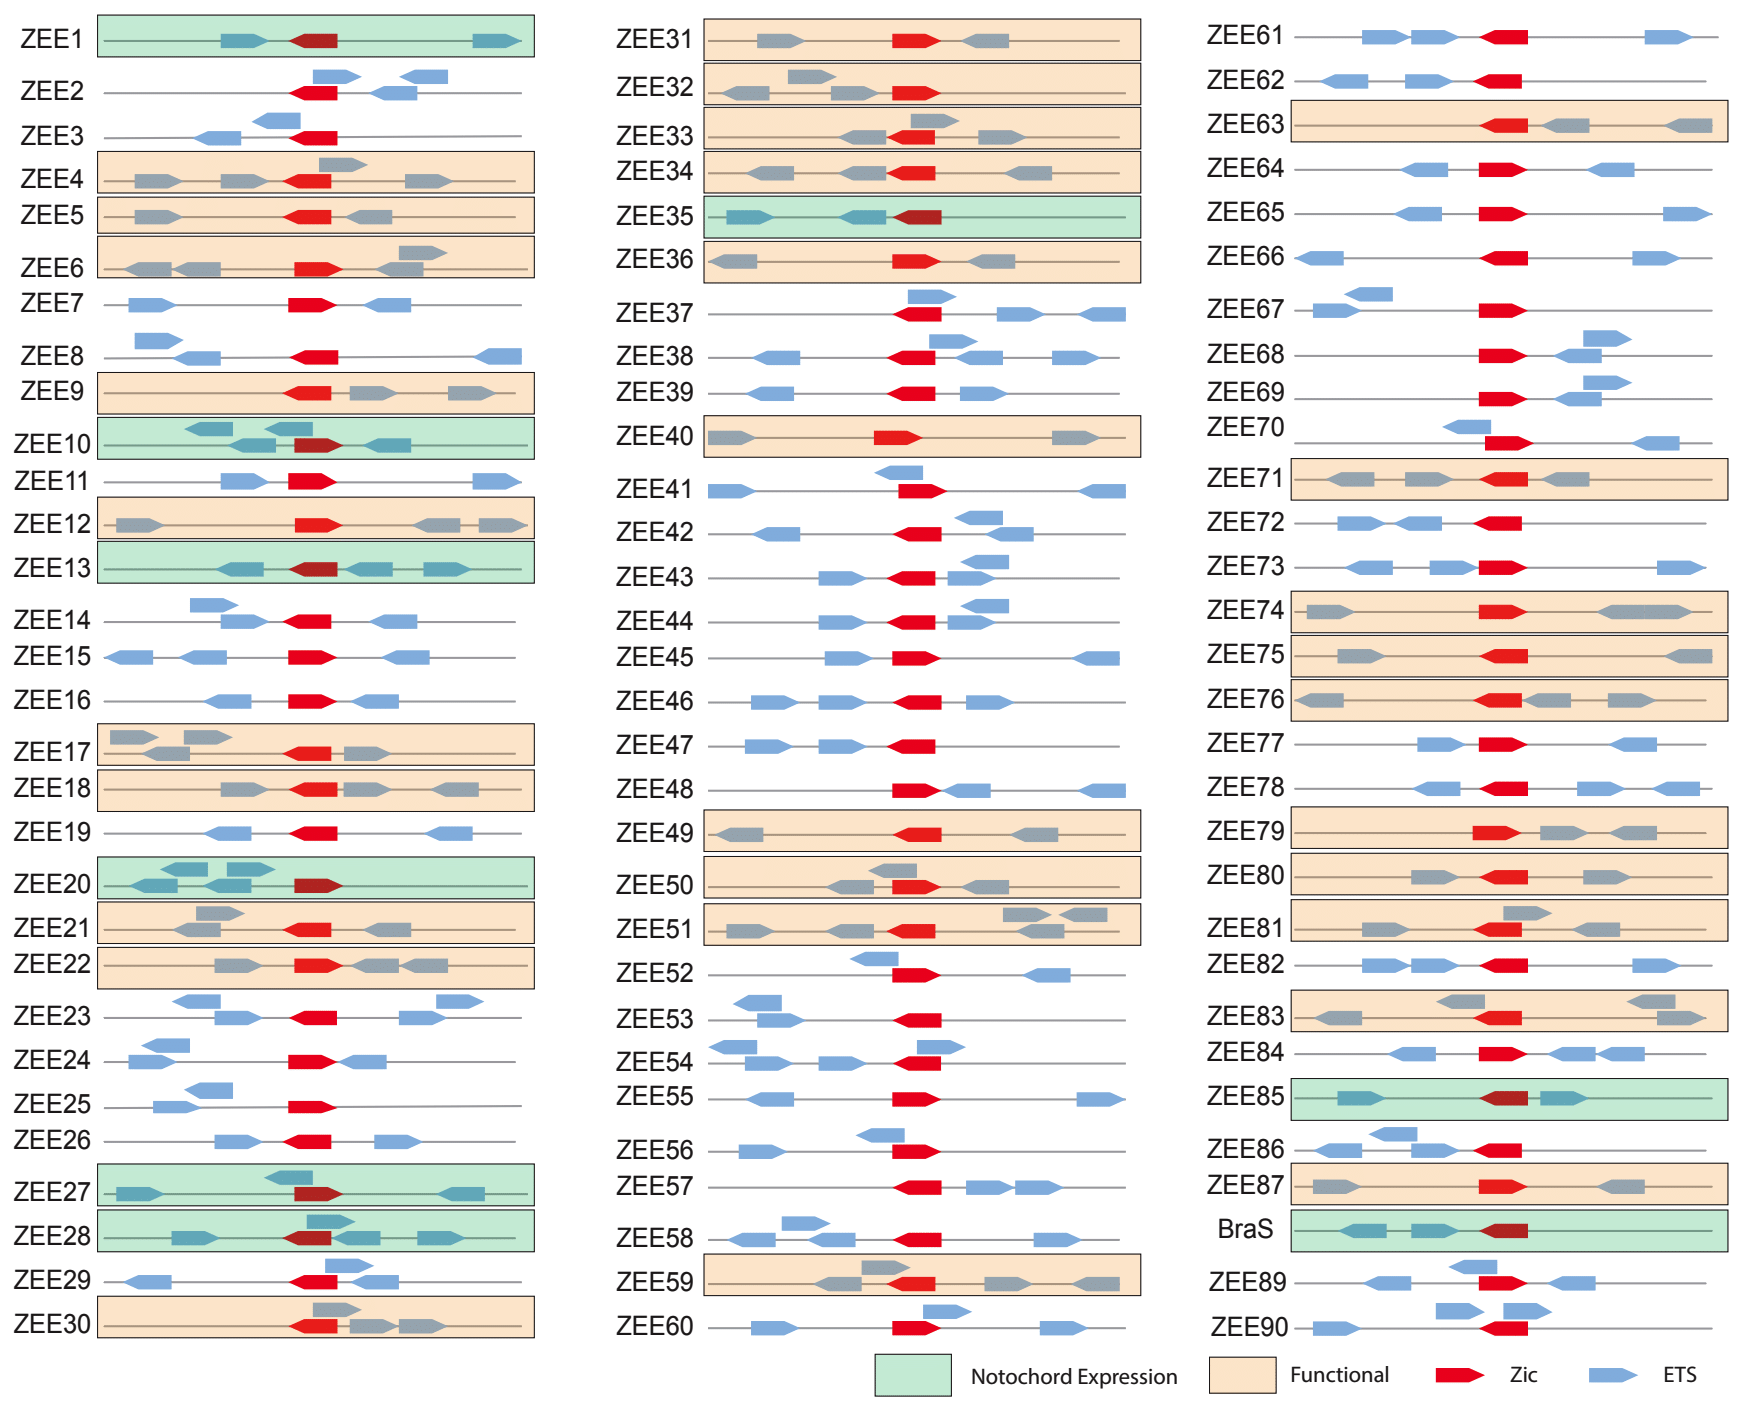
\includegraphics[scale=.2]{1_figures-and-files/FigS1_ZEE-Library.png}
    \caption[Figure title]{\textbf{Figure title.} Text here.}
    \label{fig:supplement tag for table of contents}
\end{figure}


%%%%%%%%%%%% Example of a split figure.
\begin{figure}[p]
    \centering
    \caption[Figure title]{Text here (\textit{Continued on next page.})}
    \label{fig:supplement tag2 for table of contents}
\end{figure}

\addtocounter{figure}{-1}

\captionsetup[figure]{list=no}
\begin{figure}[p]
    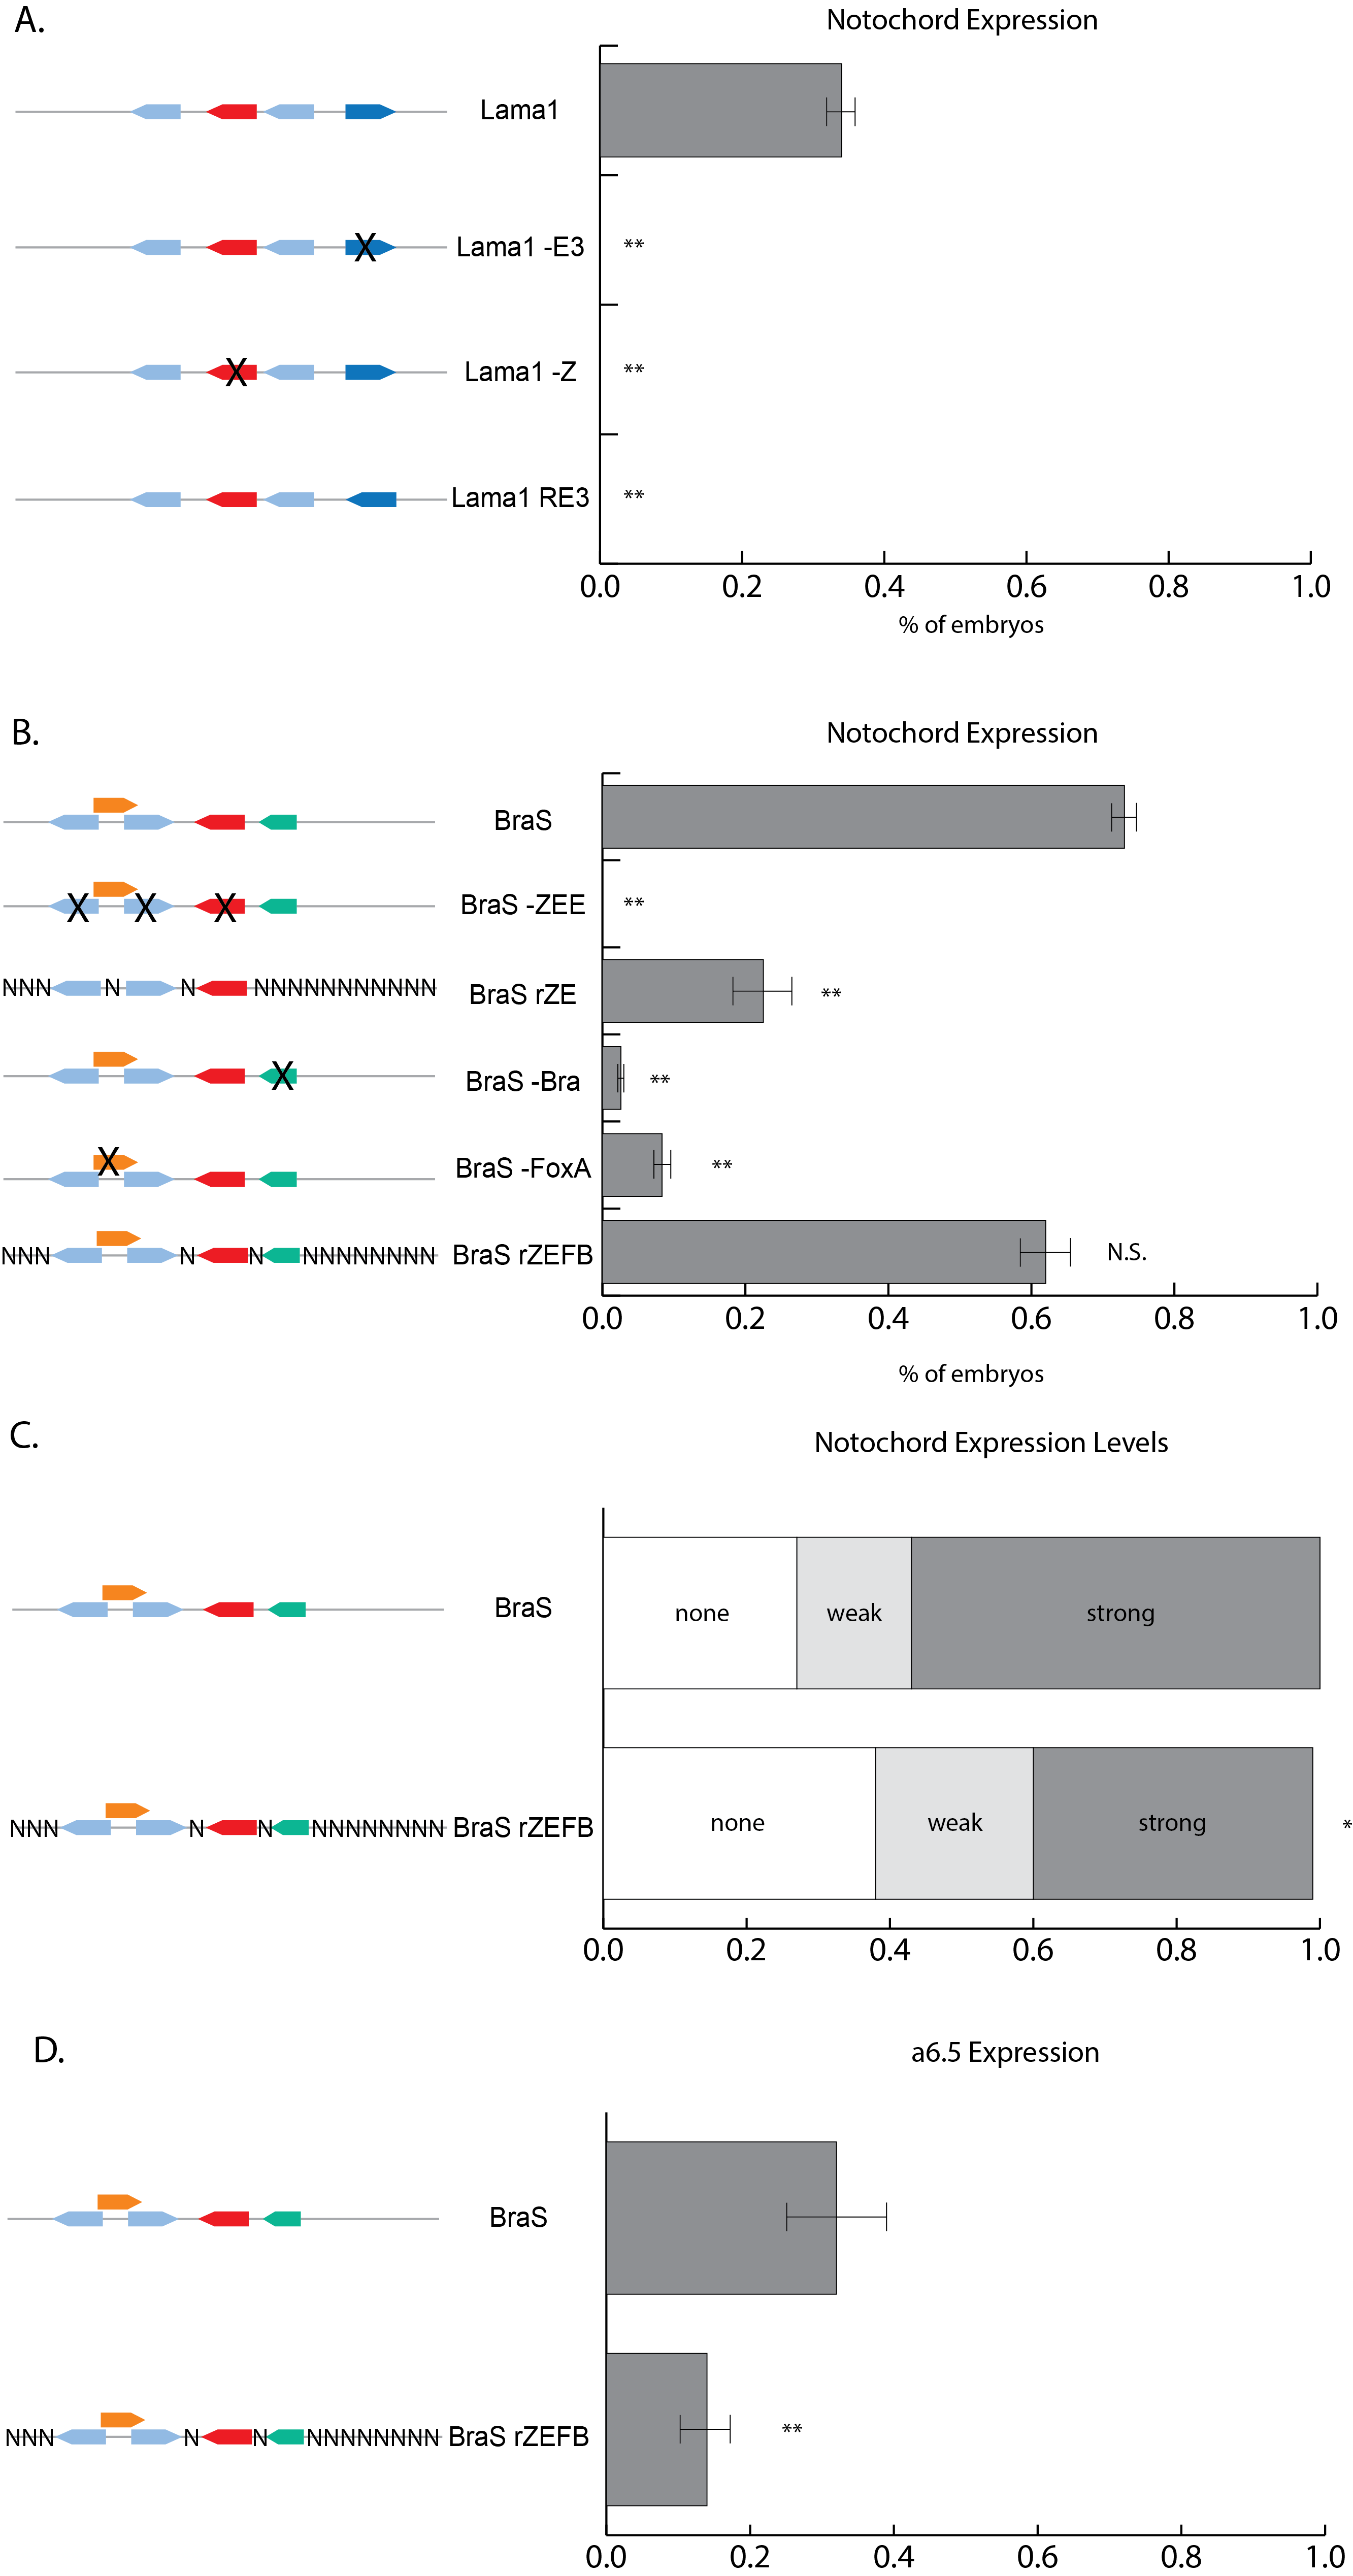
\includegraphics[scale=.5]{1_figures-and-files/FigS5_Notochord-Counting.png}
    \caption{(\textit{Continued from previous page.})}
\end{figure}
\captionsetup[figure]{list=yes}
%%%%%%%%%%%%
\appendix{}

\chapter{Supplemental Material for Chapter \ref{chap:Title of second chapter}}

%%%%%%%%%%%%%%%%%%%%%%%%%%%%%%%%%%%%%%%%%%%%%%%%%%%%%%%%%%%%%%%%%%%%%%%%%%%%%%%%
\section{Section name}
%%%%%%%%%%%%%%%%%%%%%%%%%%%%%%%%%%%%%%%%%%%%%%%%%%%%%%%%%%%%%%%%%%%%%%%%%%%%%%%%

\subsection{Subsection name}
Text here.

%%%%%%%%%%%%%%%%%%%%%%%%%%%%%%%%%%%%%%%%%%%%%%%%%%%%%%%%%%%%%%%%%%%%%%%%%%%%%%%%
\section{Supplementary Table Captions}
%%%%%%%%%%%%%%%%%%%%%%%%%%%%%%%%%%%%%%%%%%%%%%%%%%%%%%%%%%%%%%%%%%%%%%%%%%%%%%%%

The Supplemental Table can be found on the GitHub repository for this study labeled as \verb|SupplementaryTable.xlsx| at the following location: 

\noindent \href{https://github.com/Github/RepoName/}{\texttt{https://github.com/Github/RepoName/}}.

\par\noindent\dotfill

\subsubsection{Supplementary Table S1: Table title}
Text here.

%%%%%%%%%%%%%%%%%%%%%%%%%%%%%%%%%%%%%%%%%%%%%%%%%%%%%%%%%%%%%%%%%%%%%%%%%%%%%%%%
\section{Supplementary Figures}
%%%%%%%%%%%%%%%%%%%%%%%%%%%%%%%%%%%%%%%%%%%%%%%%%%%%%%%%%%%%%%%%%%%%%%%%%%%%%%%%

\begin{figure}[h]
    \centering
    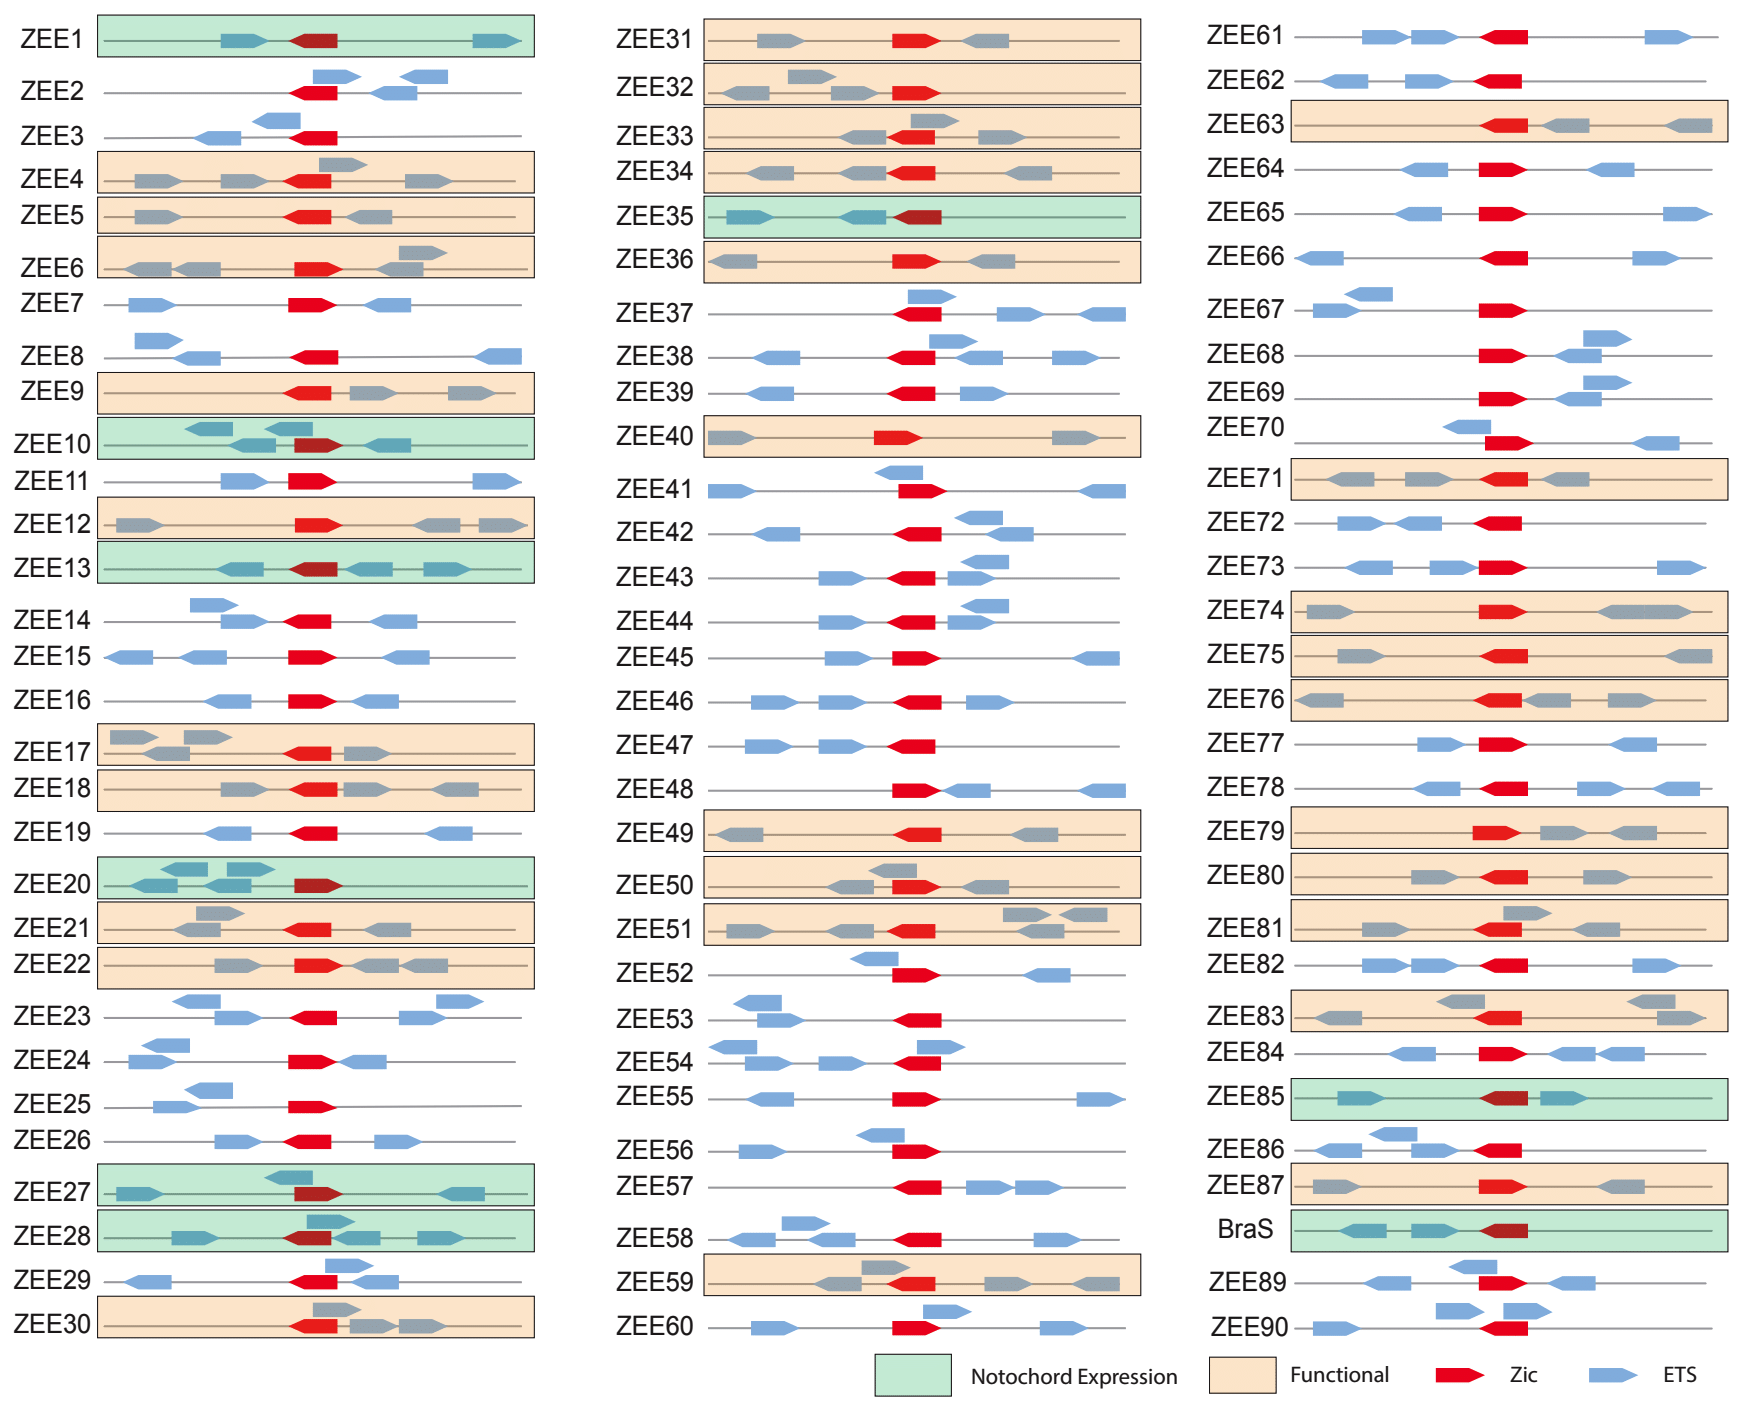
\includegraphics[scale=.2]{1_figures-and-files/FigS1_ZEE-Library.png}
    \caption[Figure title]{\textbf{Figure title.} Text here.}
    \label{fig:supplement tag for table of contents}
\end{figure}


%%%%%%%%%%%% Example of a split figure.
\begin{figure}[p]
    \centering
    \caption[Figure title]{Text here (\textit{Continued on next page.})}
    \label{fig:supplement tag2 for table of contents}
\end{figure}

\addtocounter{figure}{-1}

\captionsetup[figure]{list=no}
\begin{figure}[p]
    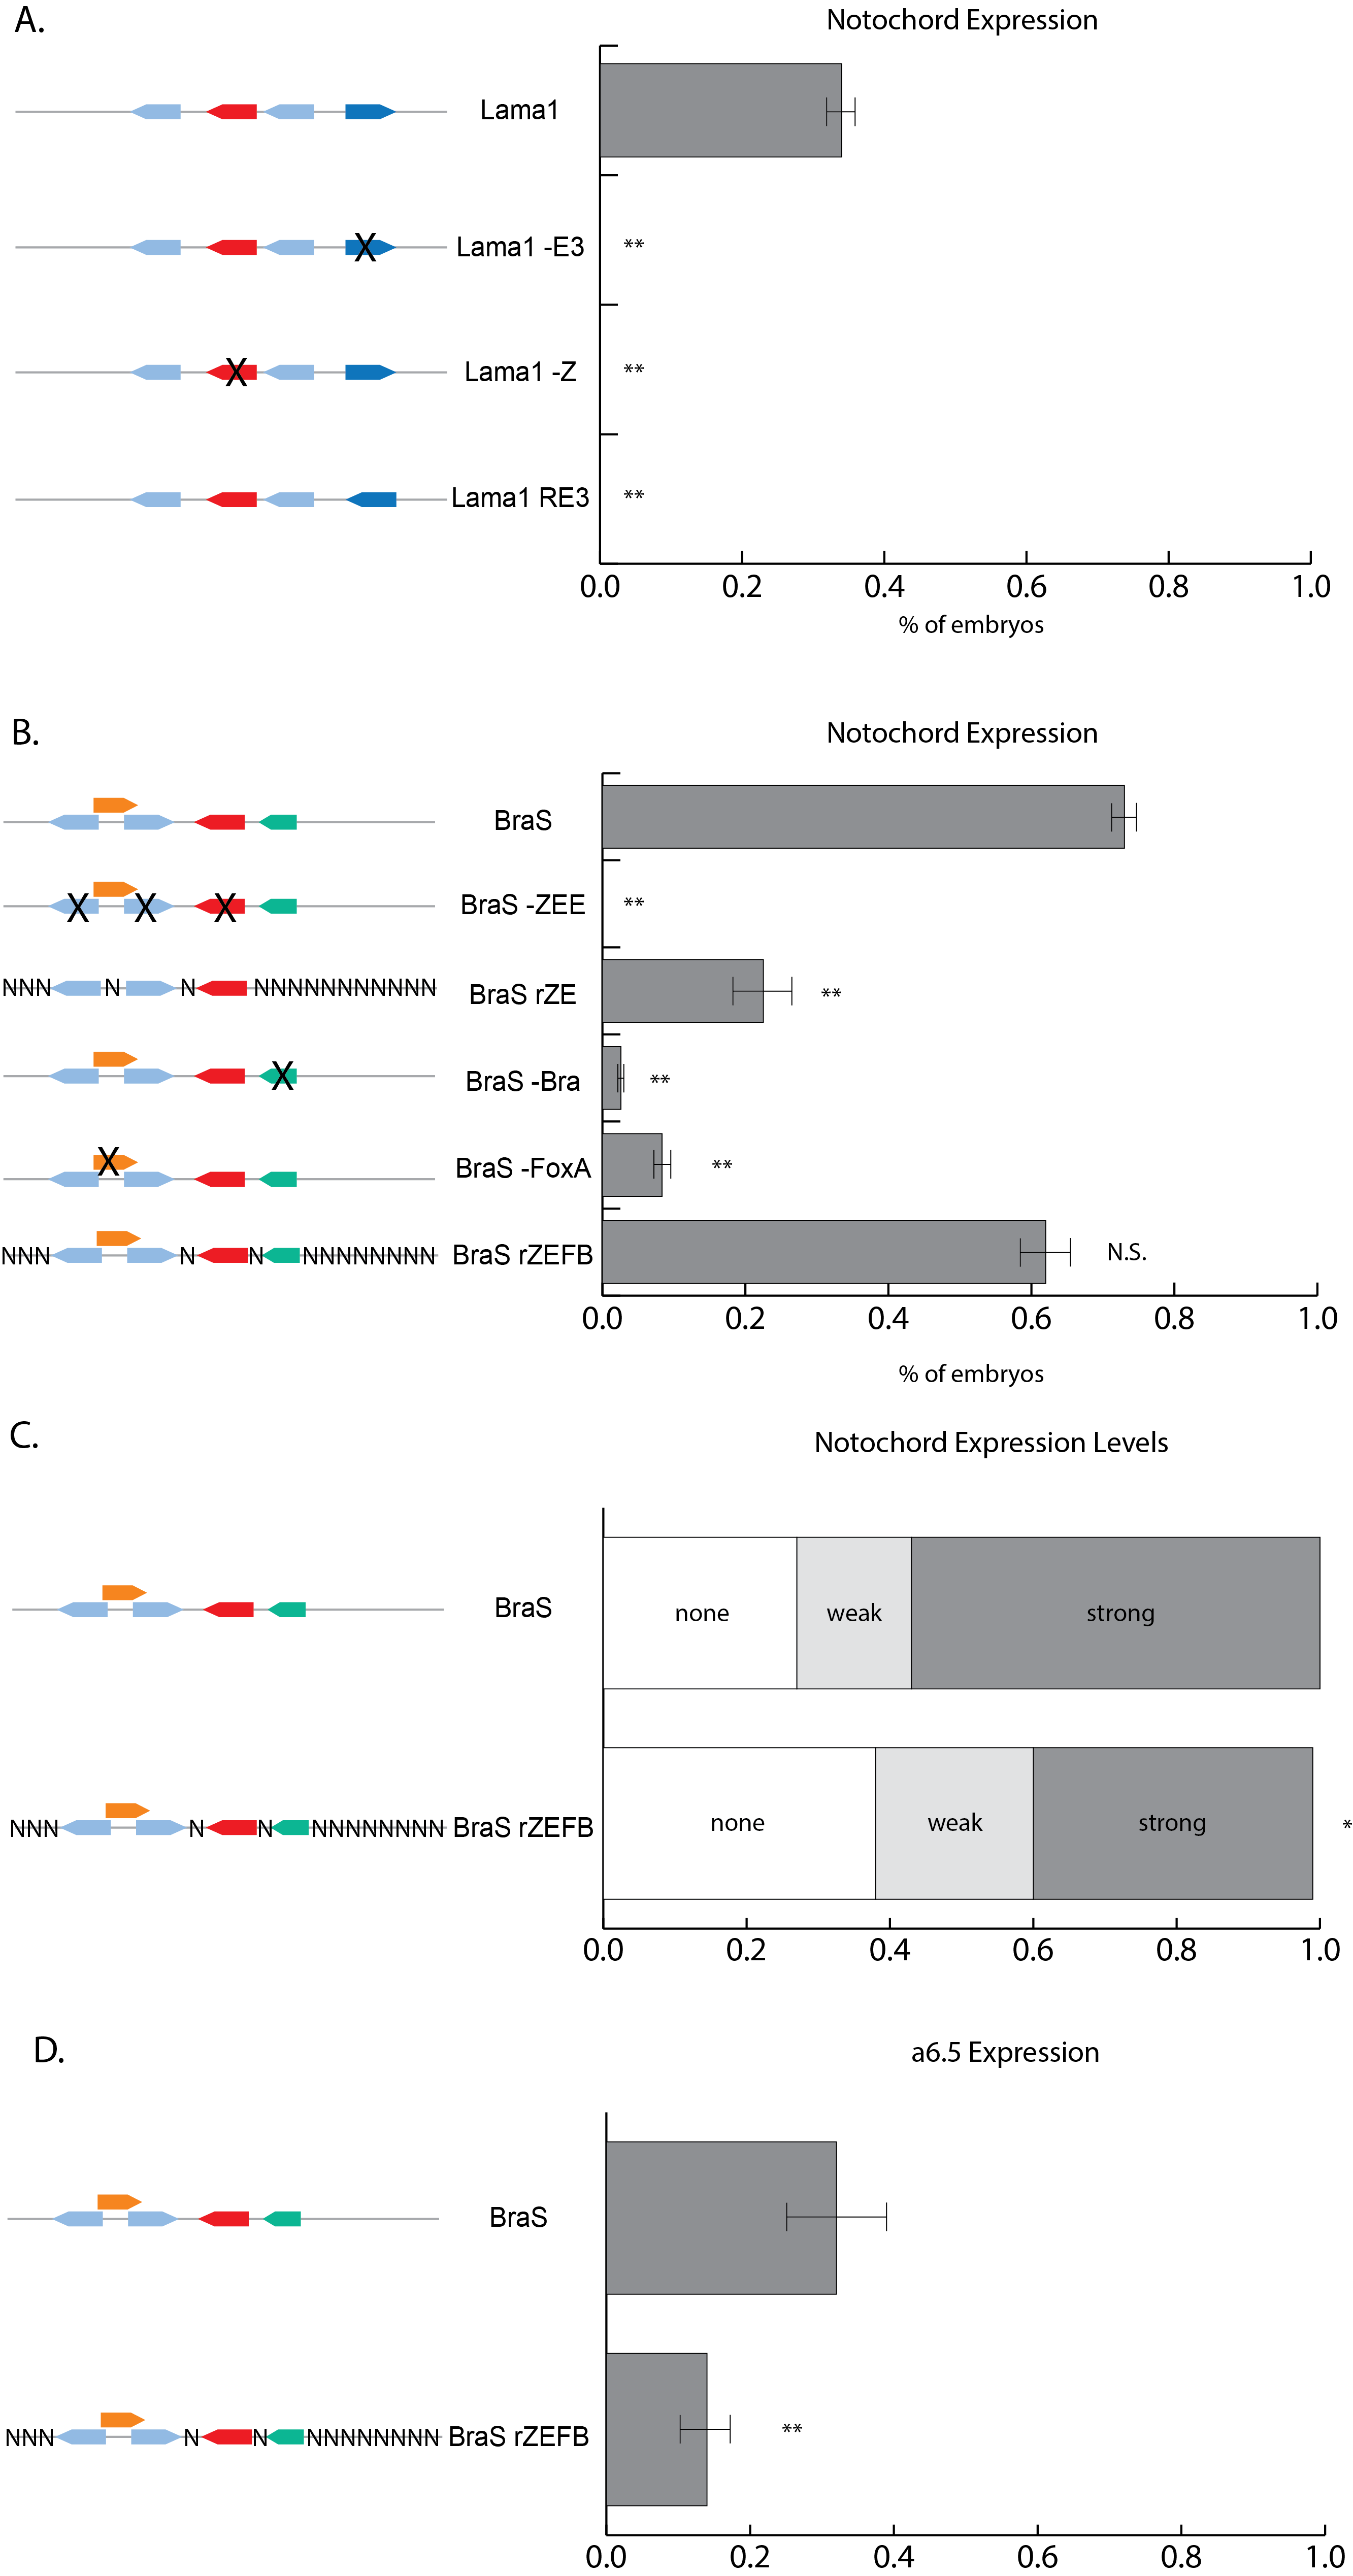
\includegraphics[scale=.5]{1_figures-and-files/FigS5_Notochord-Counting.png}
    \caption{(\textit{Continued from previous page.})}
\end{figure}
\captionsetup[figure]{list=yes}
%%%%%%%%%%%%
\appendix{}

\chapter{Supplemental Material for Chapter \ref{chap:Title of third chapter}}

%%%%%%%%%%%%%%%%%%%%%%%%%%%%%%%%%%%%%%%%%%%%%%%%%%%%%%%%%%%%%%%%%%%%%%%%%%%%%%%%
\section{Section name}
%%%%%%%%%%%%%%%%%%%%%%%%%%%%%%%%%%%%%%%%%%%%%%%%%%%%%%%%%%%%%%%%%%%%%%%%%%%%%%%%

\subsection{Subsection name}
Text here.

%%%%%%%%%%%%%%%%%%%%%%%%%%%%%%%%%%%%%%%%%%%%%%%%%%%%%%%%%%%%%%%%%%%%%%%%%%%%%%%%
\section{Supplementary Table Captions}
%%%%%%%%%%%%%%%%%%%%%%%%%%%%%%%%%%%%%%%%%%%%%%%%%%%%%%%%%%%%%%%%%%%%%%%%%%%%%%%%

The Supplemental Table can be found on the GitHub repository for this study labeled as \verb|SupplementaryTable.xlsx| at the following location: 

\noindent \href{https://github.com/Github/RepoName/}{\texttt{https://github.com/Github/RepoName/}}.

\par\noindent\dotfill

\subsubsection{Supplementary Table S1: Table title}
Text here.

%%%%%%%%%%%%%%%%%%%%%%%%%%%%%%%%%%%%%%%%%%%%%%%%%%%%%%%%%%%%%%%%%%%%%%%%%%%%%%%%
\section{Supplementary Figures}
%%%%%%%%%%%%%%%%%%%%%%%%%%%%%%%%%%%%%%%%%%%%%%%%%%%%%%%%%%%%%%%%%%%%%%%%%%%%%%%%

\begin{figure}[h]
    \centering
    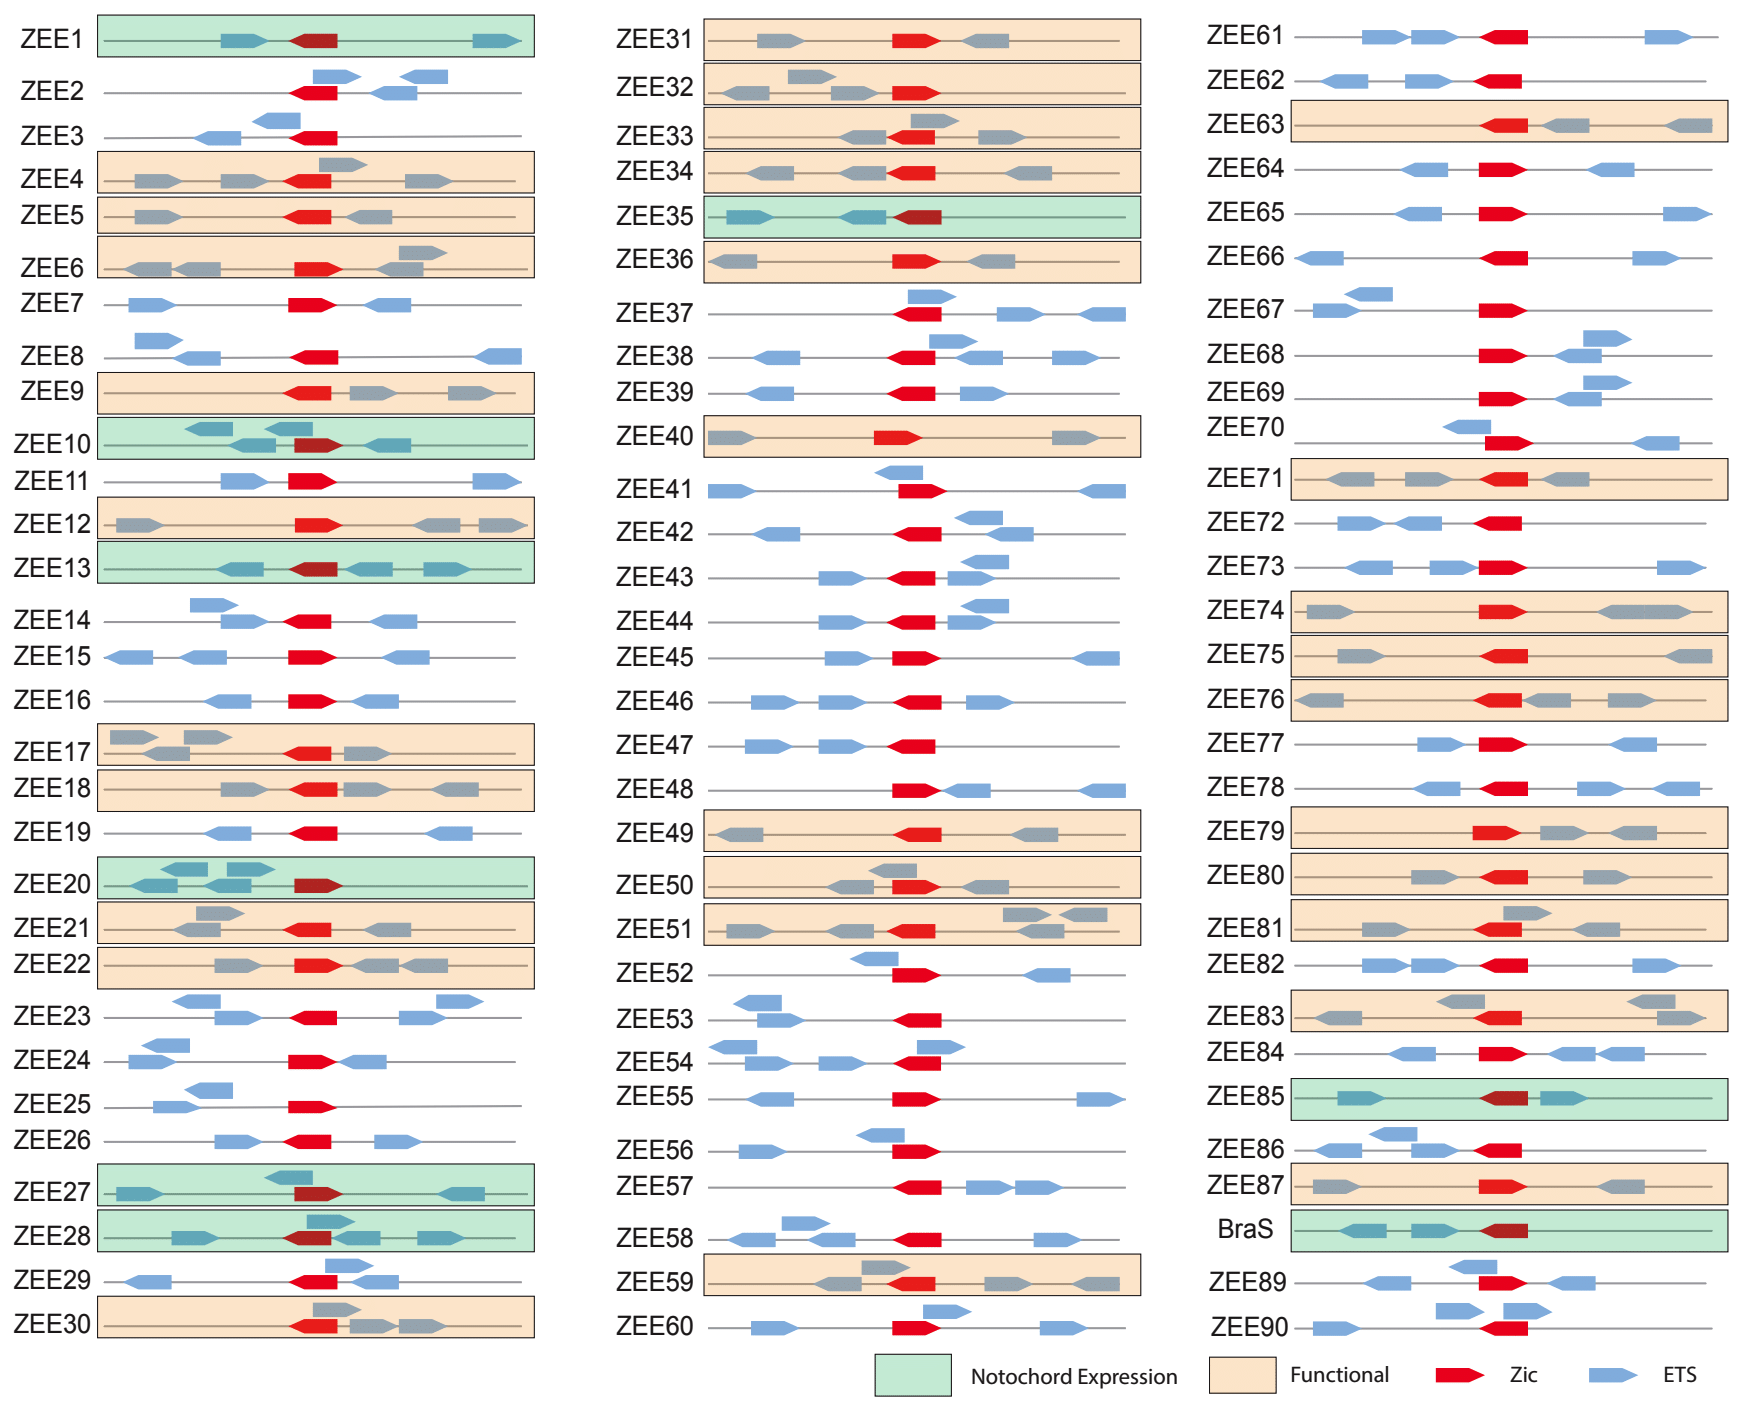
\includegraphics[scale=.2]{1_figures-and-files/FigS1_ZEE-Library.png}
    \caption[Figure title]{\textbf{Figure title.} Text here.}
    \label{fig:supplement tag for table of contents}
\end{figure}


%%%%%%%%%%%% Example of a split figure.
\begin{figure}[p]
    \centering
    \caption[Figure title]{Text here (\textit{Continued on next page.})}
    \label{fig:supplement tag2 for table of contents}
\end{figure}

\addtocounter{figure}{-1}

\captionsetup[figure]{list=no}
\begin{figure}[p]
    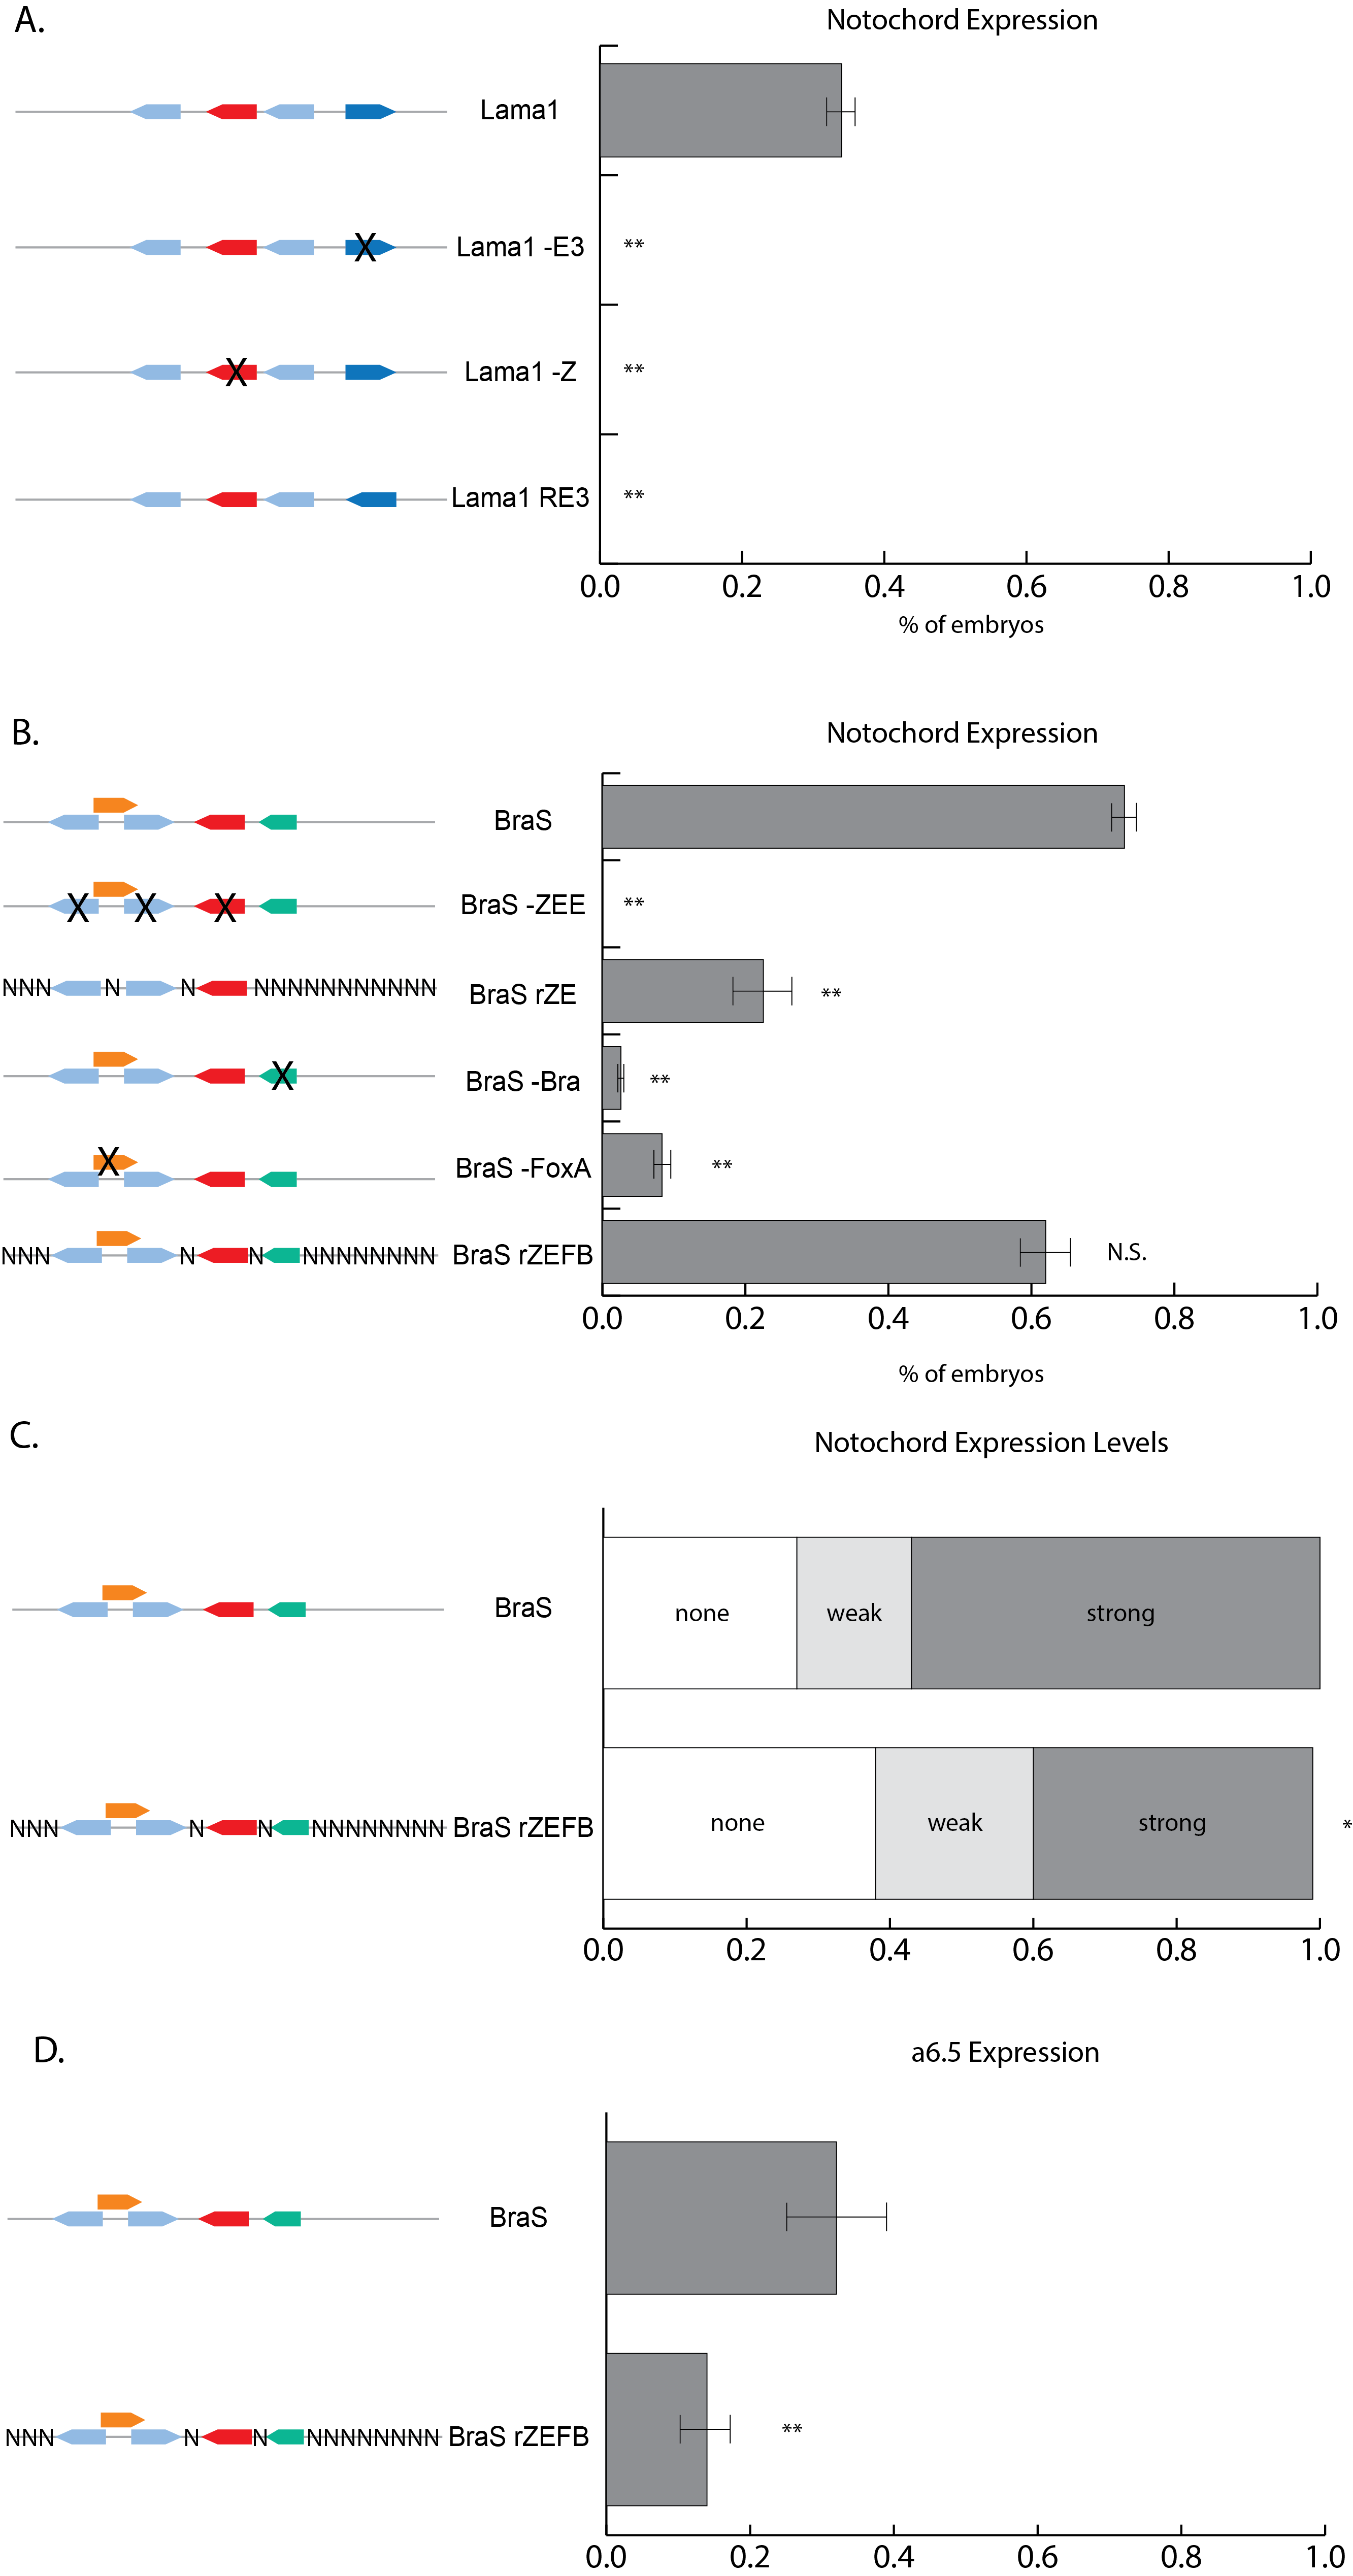
\includegraphics[scale=.5]{1_figures-and-files/FigS5_Notochord-Counting.png}
    \caption{(\textit{Continued from previous page.})}
\end{figure}
\captionsetup[figure]{list=yes}
%%%%%%%%%%%%

%%%%%%%%%%%%%%%%%%%%%%%%%%%%%%%%%%%%%%%%%%%%%%%%%%%%%%%%%%%%%%%%%%%%%%%%%%%%%%%%
% End of the Dissertation
%%%%%%%%%%%%%%%%%%%%%%%%%%%%%%%%%%%%%%%%%%%%%%%%%%%%%%%%%%%%%%%%%%%%%%%%%%%%%%%%
\backmatter{}
\bibliographystyle{unsrtnat} 
\bibliography{bibliography}

\end{document}
